\documentclass{jarfin}

\providecommand{\textLaTeX}{\LaTeX}

\graphicspath{{./3_Images/}}

\begin{document}

% ==============================
% FRONTESPIZIO
% ==============================
\input{1_Frontmatter/titlepage.tex}

% ==============================
% ABSTRACT
% ==============================
\input{1_Frontmatter/abstract.tex}

\newpage

% ==============================
% INDICI
% ==============================
\tableofcontents

\newpage

% ==============================
% CAPITOLI
% ==============================

% 1. Introduzione (Il file che hai fatto tu)
\chapter{Introduzione}

\section{Contesto e motivazione}

Negli ultimi anni, la progettazione di sistemi software complessi ha registrato una progressiva transizione da architetture monolitiche verso architetture distribuite basate su servizi indipendenti. 
Tale evoluzione è stata guidata dall’esigenza di realizzare sistemi più scalabili, manutenibili e capaci di adattarsi a requisiti in continua evoluzione.

In questo contesto, l’architettura a microservizi si è affermata come uno dei paradigmi più rilevanti. 
Essa propone la scomposizione di un’applicazione in un insieme di servizi autonomi, ciascuno responsabile di una specifica funzionalità e comunicante tramite interfacce ben definite. 
Questo approccio consente di ridurre l’accoppiamento tra componenti, facilitare l’evoluzione incrementale del sistema e migliorare la resilienza complessiva dell’architettura \cite{fowlerMicroservices}.

Parallelamente, la diffusione di tecnologie web standard ha favorito l’adozione di modelli architetturali basati su API REST (Representational State Transfer), che costituiscono uno stile architetturale ampiamente utilizzato per la comunicazione tra sistemi distribuiti. 
Le API REST si basano su interazioni stateless, risorse identificabili e interfacce uniformi, favorendo interoperabilità e semplicità di integrazione tra componenti eterogenei \cite{fieldingRest}.

Un ulteriore sviluppo significativo riguarda l’integrazione di interfacce conversazionali, che consentono agli utenti di interagire con i sistemi software tramite linguaggio naturale. 
Questo paradigma migliora l’accessibilità e l’usabilità delle applicazioni, riducendo la complessità dell’interazione e rendendo i sistemi più intuitivi anche per utenti non esperti \cite{nlpSurvey}.

Nel dominio delle applicazioni per la gestione delle finanze personali, l’adozione combinata di architetture a microservizi, API REST e interfacce conversazionali apre nuove opportunità per la progettazione di sistemi modulari, scalabili e orientati all’utente, capaci di integrare funzionalità avanzate di analisi dei dati e di interazione.

\section{Problema}

I sistemi tradizionali per la gestione delle finanze personali presentano spesso limitazioni architetturali e funzionali. 
In particolare, molti di essi sono progettati come applicazioni monolitiche, caratterizzate da un forte accoppiamento tra componenti e da una limitata separazione delle responsabilità. 
Questo approccio rende complessa l’evoluzione del sistema, ostacola la manutenzione del codice e limita l’introduzione di nuove funzionalità.

Inoltre, l’interazione con tali sistemi avviene prevalentemente tramite interfacce grafiche tradizionali, che richiedono all’utente di navigare manualmente tra diverse schermate e inserire dati in modo strutturato. 
Questo approccio risulta spesso poco intuitivo e inefficiente, in particolare per utenti non esperti o in presenza di un elevato numero di operazioni da gestire.

Dal punto di vista dell’esperienza utente, tali modalità di interazione introducono ulteriori criticità. 
L’inserimento manuale delle transazioni tramite form strutturati comporta un elevato carico cognitivo e operativo: la necessità di specificare categorie, importi e date per ogni singola operazione richiede tempo e attenzione, riducendo la probabilità di un utilizzo continuativo dell’applicazione nel lungo periodo.

In molti casi, l’utente è costretto ad adattarsi al modello dati del software, piuttosto che interagire secondo il proprio modello mentale. 
Manca infatti un approccio \textit{frictionless} che consenta di registrare una spesa o interrogare i propri dati finanziari con la stessa naturalezza con cui tali informazioni vengono comunicate verbalmente.

Dal punto di vista architetturale, la mancanza di modularità limita inoltre la scalabilità del sistema e ne riduce la robustezza, rendendo più complessa l’integrazione con nuovi servizi e l’evoluzione futura dell’applicazione.

Pertanto, emerge la necessità di progettare un sistema software che consenta di:
\begin{itemize}
\item gestire le finanze personali in modo strutturato e affidabile;
\item garantire modularità e separazione delle responsabilità;
\item supportare architetture distribuite scalabili;
\item fornire un’interfaccia utente intuitiva, inclusa l’interazione tramite linguaggio naturale;
\item consentire un’analisi efficiente dei dati finanziari.
\end{itemize}

\section{Obiettivi del progetto}

L’obiettivo del presente lavoro è la progettazione e lo sviluppo di \textit{JarFin} (Java Artificial Financial Intelligence), un sistema software distribuito per la gestione e l’analisi delle finanze personali, basato su un’architettura a microservizi.

Gli obiettivi specifici del progetto includono:
\begin{itemize}
\item la progettazione di un’architettura software modulare basata su microservizi;
\item la realizzazione di servizi indipendenti per la gestione delle transazioni e l’analisi dei dati;
\item l’implementazione di un sistema di comunicazione basato su API REST;
\item l’integrazione di un modulo di Natural Language Understanding per l’elaborazione di comandi in linguaggio naturale;
\item la realizzazione di un’interfaccia web per l’interazione con il sistema;
\item l’applicazione di principi di progettazione algoritmica e modellazione software.
\end{itemize}

\section{Soluzione proposta}

Per soddisfare gli obiettivi definiti, è stato progettato e sviluppato JarFin come sistema distribuito basato su architettura a microservizi.

Il sistema è composto dai seguenti componenti principali:
\begin{itemize}
\item \textbf{Web Application}, che rappresenta l’interfaccia utente e consente l’interazione con il sistema tramite browser;
\item \textbf{API Gateway}, che funge da punto di accesso centralizzato e gestisce l’instradamento delle richieste verso i microservizi appropriati;
\item \textbf{Accounting Service}, responsabile della gestione e della persistenza delle transazioni finanziarie all’interno di un database PostgreSQL;
\item \textbf{Analytics Service}, che elabora i dati finanziari e genera report e statistiche;
\item \textbf{NLU Service}, che consente l’elaborazione di comandi in linguaggio naturale e la loro traduzione in operazioni eseguibili;
\item \textbf{Database PostgreSQL}, che garantisce la persistenza e l’integrità dei dati.
\end{itemize}

La comunicazione tra i componenti avviene tramite API REST e scambio di dati in formato JSON, secondo i principi architetturali definiti nello stile REST \cite{fieldingRest}. 
L’utilizzo del framework Spring Boot consente lo sviluppo di microservizi indipendenti e facilmente configurabili, migliorando la modularità e la manutenibilità complessiva del sistema \cite{springboot}.

L’architettura complessiva del sistema è illustrata nel diagramma di alto livello presentato nei capitoli successivi, che evidenzia le relazioni tra i diversi microservizi e il ruolo centrale dell’API Gateway.

\section{Contributi del lavoro}

I principali contributi del presente lavoro includono:
\begin{itemize}
\item la progettazione e validazione di un’architettura software distribuita basata su microservizi per la gestione delle finanze personali;
\item l’integrazione di un modulo di Natural Language Understanding in un sistema finanziario reale, consentendo l’interazione tramite linguaggio naturale;
\item la realizzazione di un flusso completo di acquisizione, elaborazione e analisi dei dati finanziari tramite servizi indipendenti;
\item l’adozione di un’architettura basata su API REST e API Gateway per migliorare la scalabilità e ridurre l’accoppiamento tra componenti;
\item l’applicazione di principi di progettazione algoritmica e architetturale in un contesto concreto e funzionante;
\item la validazione dell’approccio proposto attraverso implementazione e testing.
\end{itemize}

\newpage
\section{Struttura del documento}

Il presente elaborato è organizzato seguendo l’iter di sviluppo del progetto:
\begin{itemize}
\item Il \textbf{Capitolo 2} presenta il contesto metodologico adottato (SCRUM/AMDD) e la toolchain tecnologica utilizzata;
\item Il \textbf{Capitolo 3} (Iterazione 0) descrive l’analisi dei requisiti e l’architettura del sistema secondo il modello 4+1;
\item Il \textbf{Capitolo 4} (Iterazione 1) presenta l’implementazione dei servizi core e la gestione della persistenza;
\item Il \textbf{Capitolo 5} (Iterazione 2) analizza gli algoritmi di business intelligence e il servizio di analytics;
\item Il \textbf{Capitolo 6} (Iterazione 3) descrive l’integrazione del modulo NLU, dell’API Gateway e dell’interfaccia utente;
\item Il \textbf{Capitolo 7} presenta le attività di testing e la validazione dell’architettura;
\item Il \textbf{Capitolo 8} riporta le conclusioni e le possibili evoluzioni future del sistema.
\end{itemize}

% 2. Metodologia (Processo Scrum, AMDD, Toolchain)
\chapter{Metodologia di sviluppo e tecnologie adottate}

\section{Metodologia di sviluppo}

Lo sviluppo del sistema \textit{JarFin} è stato condotto adottando una metodologia Agile, con l’obiettivo di favorire un processo di progettazione incrementale, flessibile e orientato al cambiamento. In particolare, il progetto ha seguito i principi di \textbf{SCRUM}, integrati con l’approccio \textbf{Agile Model Driven Development (AMDD)}, al fine di bilanciare la necessità di una progettazione architetturale solida con i vantaggi dell’iterazione continua e del feedback costante.

SCRUM è stato utilizzato come framework di riferimento per l’organizzazione del lavoro, la pianificazione delle attività e la gestione delle iterazioni di sviluppo. Il ciclo di vita del progetto è stato articolato in sprint di durata indicativa pari a due settimane, ciascuno caratterizzato da obiettivi ben definiti e dalla produzione di un incremento funzionale del sistema. Questa impostazione ha consentito di monitorare costantemente l’avanzamento del progetto e di adattare le scelte progettuali in base alle esigenze emerse durante lo sviluppo \cite{scrum}.

Parallelamente, l’approccio AMDD ha guidato le attività di modellazione e progettazione. Invece di definire in modo esaustivo l’intera architettura nelle fasi iniziali, la modellazione è stata condotta in maniera incrementale, producendo modelli essenziali e sufficienti a supportare le decisioni architetturali di ciascuna iterazione. In particolare, sono stati realizzati modelli di dominio e diagrammi UML (use case, componenti, classi e sequenza) per i casi d’uso più rilevanti, successivamente raffinati nel corso dello sviluppo \cite{amdd}. Questo approccio ha permesso di evitare un’eccessiva rigidità progettuale, mantenendo al contempo una visione coerente dell’architettura complessiva del sistema.

\section{Organizzazione delle iterazioni}

Il ciclo di sviluppo di JarFin è stato articolato in una serie di iterazioni successive, ciascuna focalizzata su specifici obiettivi funzionali e architetturali:

\begin{itemize}
\item \textbf{Iterazione 0 – Envisioning e Analisi}: definizione del dominio applicativo, raccolta e analisi dei requisiti funzionali e non funzionali, identificazione dei principali casi d’uso e progettazione dell’architettura di alto livello;
\item \textbf{Iterazione 1 – Core Services}: progettazione e implementazione dei servizi fondamentali del sistema, con particolare riferimento al servizio di accounting e alla gestione della persistenza dei dati;
\item \textbf{Iterazione 2 – Analytics e Algoritmi}: sviluppo del servizio di analytics e implementazione degli algoritmi per l’elaborazione e l’analisi dei dati finanziari;
\item \textbf{Iterazione 3 – Integrazione e Interazione}: integrazione del modulo di Natural Language Understanding, dell’API Gateway e dell’interfaccia web.
\end{itemize}

Questa suddivisione ha consentito di affrontare progressivamente la complessità del sistema, validando le scelte progettuali a ogni iterazione e riducendo il rischio di errori architetturali nelle fasi avanzate dello sviluppo.

\section{Architettura generale del sistema}

L’architettura di JarFin è basata su un paradigma a microservizi, in cui il sistema è scomposto in un insieme di componenti indipendenti, ciascuno responsabile di una specifica area funzionale. Tale scelta architetturale è motivata dall’esigenza di garantire modularità, scalabilità e manutenibilità, oltre a facilitare l’evoluzione futura del sistema.

Ogni microservizio è progettato come un’unità autonoma, dotata di una propria logica applicativa e, ove necessario, di un proprio livello di persistenza. La comunicazione tra i servizi avviene tramite API REST e scambio di messaggi in formato JSON, secondo i principi dello stile architetturale REST \cite{fieldingRest}.

L’adozione di un’architettura distribuita consente inoltre di isolare le responsabilità dei singoli componenti, riducendo l’impatto delle modifiche e migliorando la resilienza complessiva del sistema in caso di malfunzionamenti localizzati.

\section{Tecnologie adottate}

La scelta dello stack tecnologico è stata guidata dalla necessità di utilizzare strumenti robusti, ampiamente supportati dalla community e adatti allo sviluppo di sistemi distribuiti.

\subsection{Spring Boot}

Per l’implementazione dei microservizi è stato utilizzato il framework \textbf{Spring Boot}, che fornisce un ambiente di sviluppo semplificato per la realizzazione di applicazioni Java basate su architettura a servizi. Spring Boot consente di ridurre significativamente la configurazione manuale, favorendo lo sviluppo rapido di applicazioni standalone e facilmente deployabili \cite{springboot}.

Il framework supporta nativamente la creazione di API REST, l’integrazione con sistemi di persistenza e la gestione della configurazione dei servizi, risultando particolarmente adatto allo sviluppo di architetture a microservizi.

\subsection{Database PostgreSQL}

La persistenza dei dati è affidata a un database relazionale \textbf{PostgreSQL}, scelto per la sua affidabilità, conformità agli standard SQL e supporto a funzionalità avanzate di gestione dei dati. PostgreSQL garantisce l’integrità dei dati finanziari e supporta operazioni di interrogazione efficienti, fondamentali per le funzionalità di analisi offerte dal sistema.

\subsection{Modulo di Natural Language Understanding}

Per l’elaborazione del linguaggio naturale è stato sviluppato un modulo di Natural Language Understanding implementato in Java come microservizio dedicato. Il sistema utilizza tecniche di analisi lessicale e \textit{pattern matching} per identificare intenti e parametri rilevanti a partire dalle frasi dell’utente, consentendo l’esecuzione di operazioni finanziarie tramite comandi in linguaggio naturale.

La scelta di una soluzione interna, anziché basata su servizi cloud esterni, consente di ridurre la latenza, mantenere il controllo sui dati sensibili dell’utente e garantire una maggiore integrazione con l’architettura complessiva del sistema.

\subsection{Containerizzazione e ambiente di esecuzione}

Per facilitare il deployment e garantire la riproducibilità dell’ambiente di esecuzione, il sistema è stato containerizzato mediante \textbf{Docker}. L’utilizzo di container consente di isolare i singoli microservizi e le relative dipendenze, semplificando la gestione dell’infrastruttura e favorendo la portabilità del sistema tra ambienti di sviluppo e produzione.

\section{Toolchain di progetto}

Lo sviluppo del sistema \textit{JarFin} è stato supportato da una toolchain articolata, composta da strumenti dedicati alla modellazione, allo sviluppo, al versioning, al testing e all’analisi della qualità del codice.  
La scelta degli strumenti è stata guidata dall’obiettivo di garantire un processo di sviluppo strutturato, tracciabile e conforme alle buone pratiche dell’ingegneria del software.

\subsection{Strumenti di modellazione}

Per la modellazione del sistema è stato utilizzato \textbf{UMLet}, uno strumento leggero per la creazione di diagrammi UML. UMLet è stato impiegato per la realizzazione dei principali artefatti di modellazione previsti dall’approccio AMDD, in particolare:
\begin{itemize}
\item diagrammi dei casi d’uso, per rappresentare le funzionalità offerte dal sistema e le interazioni con gli attori;
\item diagrammi delle classi, per descrivere la struttura statica dei principali componenti software;
\item diagrammi dei componenti, per modellare l’architettura a microservizi;
\item diagrammi di sequenza, per analizzare il comportamento dinamico del sistema nei casi d’uso critici.
\end{itemize}

L’utilizzo di UMLet ha consentito di produrre modelli essenziali e facilmente modificabili, in linea con i principi della modellazione incrementale promossi dall’Agile Model Driven Development.

\subsection{Versioning e Project Management}

Il controllo di versione del codice sorgente e la gestione del progetto sono stati affidati a \textbf{GitHub}.  
Git è stato utilizzato come sistema di versioning distribuito, permettendo di tracciare l’evoluzione del codice, gestire rami di sviluppo separati e mantenere uno storico completo delle modifiche.

GitHub è stato inoltre impiegato come strumento di supporto al project management, sfruttando:
\begin{itemize}
\item repository centralizzato per il codice sorgente;
\item Kanban board per la pianificazione delle attività e il tracciamento delle iterazioni;
\item Pull Request per la revisione del codice e l’integrazione controllata delle funzionalità.
\end{itemize}

Questa impostazione ha favorito un processo di sviluppo ordinato e trasparente, coerente con la metodologia SCRUM adottata.

\subsection{Sviluppo backend}

Il backend del sistema è stato sviluppato utilizzando il linguaggio \textbf{Java} e il framework \textbf{Spring Boot}.  
Spring Boot è stato scelto per la sua capacità di semplificare lo sviluppo di applicazioni basate su architettura a microservizi, riducendo la configurazione manuale e favorendo la realizzazione di servizi REST standalone.

Ogni microservizio di JarFin è implementato come applicazione Spring Boot indipendente, responsabile di una specifica area funzionale del sistema, in linea con i principi di separazione delle responsabilità e modularità.

\subsection{Testing delle API REST}

Per la verifica manuale e il testing degli endpoint REST è stato utilizzato \textbf{Postman}.  
Lo strumento ha permesso di:
\begin{itemize}
\item testare le operazioni CRUD esposte dai microservizi;
\item validare il corretto formato delle richieste e delle risposte JSON;
\item simulare scenari di utilizzo reali durante le fasi di sviluppo e integrazione.
\end{itemize}

L’uso di Postman ha facilitato l’individuazione precoce di errori di comunicazione tra i servizi e ha supportato la fase di debugging dell’API Gateway.

\subsection{Unit Testing}

Il testing automatico della logica applicativa è stato realizzato tramite \textbf{JUnit 5}, framework di riferimento per il testing in ambiente Java.  
JUnit è stato utilizzato per definire test unitari mirati a verificare il corretto funzionamento dei metodi di business logic, in particolare nei servizi di accounting, analytics e NLU.

L’adozione del testing unitario ha contribuito a migliorare l’affidabilità del sistema e a ridurre il rischio di regressioni durante l’evoluzione del codice.

\subsection{Analisi della copertura del codice}

Per l’analisi della copertura dei test è stato utilizzato il plugin \textbf{EclEmma}, integrato nell’ambiente di sviluppo.  
EclEmma consente di misurare dinamicamente la percentuale di codice eseguito durante l’esecuzione dei test, fornendo indicatori utili per valutare l’efficacia della suite di test.

Le metriche di copertura hanno supportato l’identificazione delle porzioni di codice meno testate, guidando il miglioramento progressivo dei test unitari.

\subsection{Analisi statica del codice}

La qualità strutturale del codice è stata analizzata mediante \textbf{STAN4J}, strumento di analisi statica per applicazioni Java.  
STAN4J è stato utilizzato per:
\begin{itemize}
\item valutare metriche di complessità e dipendenze tra classi;
\item individuare potenziali criticità architetturali;
\item supportare la verifica del rispetto dei principi di progettazione software.
\end{itemize}

L’analisi statica ha contribuito a mantenere un’architettura pulita e coerente con i principi di modularità e manutenibilità, aspetti fondamentali in un sistema a microservizi.

\subsection{Considerazioni sulla toolchain}

L’integrazione degli strumenti descritti ha permesso di coprire l’intero ciclo di vita del software, dalla modellazione iniziale alla verifica della qualità del codice.  
La toolchain adottata rappresenta una soluzione completa e coerente con gli obiettivi del progetto, fornendo un supporto efficace sia allo sviluppo incrementale sia alla validazione tecnica del sistema.

% 3. Iterazione 0 (Requisiti, Architettura 4+1)
\chapter{Analisi dei requisiti e architettura del sistema}

\section{Visione del prodotto}

\subsection{Ispirazione e contesto}

L'idea alla base del sistema \textit{JarFin} trae ispirazione dal paradigma degli assistenti intelligenti proattivi, resi popolari in ambito cinematografico da sistemi come J.A.R.V.I.S. (\textit{Just A Rather Very Intelligent System}). In tale contesto ideale, l'assistente è in grado di comprendere richieste espresse in linguaggio naturale e di eseguire operazioni complesse in modo autonomo, riducendo drasticamente il carico cognitivo dell'utente.

Nel mondo reale, tuttavia, la gestione delle finanze personali rappresenta un'attività spesso inefficiente e frammentata. Gli utenti sono costretti a utilizzare molteplici applicazioni bancarie, inserire manualmente dati in fogli di calcolo e navigare interfacce complesse (WIMP) per ottenere informazioni basilari sul proprio stato finanziario.
Questa modalità operativa introduce un'elevata "frizione", aumentando il rischio di errori di trascrizione e riducendo la frequenza con cui gli utenti monitorano le proprie finanze.

\newpage
\subsection{Obiettivi del sistema}

JarFin si propone di colmare questo divario introducendo un assistente finanziario intelligente in grado di:
\begin{itemize}
    \item comprendere comandi espressi in linguaggio naturale (NLU);
    \item trasformare input non strutturati (es. "Pizza 20 euro") in operazioni finanziarie formalmente definite;
    \item centralizzare la gestione delle transazioni finanziarie in un unico hub;
    \item fornire funzionalità avanzate di analisi e reporting automatico;
    \item garantire un'architettura scalabile, modulare ed estendibile tramite microservizi.
\end{itemize}

\section{Analisi dei requisiti}

In questa fase di \textit{Envisioning} (Iterazione 0), sono stati formalizzati i requisiti necessari per costruire il Core, l'Analytics e il modulo NLU.

\subsection{Requisiti funzionali}

I requisiti funzionali definiscono le capacità operative che il sistema deve esporre.

\begin{small}
    \begin{longtable}{|c|p{4cm}|p{6cm}|c|}

        \hline
        \textbf{ID} & \textbf{Requisito}              & \textbf{Descrizione}                                                                                                                                                                            & \textbf{Priorità} \\ \hline
        \endfirsthead

        \multicolumn{4}{c}{{}}                                                                                                                                                                                                                                              \\
        \hline
        \textbf{ID} & \textbf{Requisito}              & \textbf{Descrizione}                                                                                                                                                                            & \textbf{Priorità} \\ \hline
        \endhead

        \hline
        \endfoot

        RF-01       & Gestione transazioni (CRUD)     & Il sistema deve consentire la creazione, lettura, aggiornamento e cancellazione delle transazioni tramite API REST esposte dal servizio Accounting.                                             & Alta              \\ \hline
        RF-02       & Parsing del linguaggio naturale & Il servizio NLU deve interpretare input testuali ed estrarre le entità rilevanti (importo, categoria, tipo) utilizzando la classe \texttt{NaturalLanguageService} e il metodo \texttt{parse()}. & Alta              \\ \hline
        RF-03       & Aggregazione e reporting        & Il servizio Analytics deve aggregare i dati finanziari e generare statistiche temporali tramite la classe \texttt{DataAggregator}.                                                              & Media             \\ \hline
        RF-04       & Orchestrazione API Gateway      & Il sistema deve fornire un punto di accesso unico tramite \texttt{APIGateway}, responsabile del routing verso i microservizi.                                                                   & Alta              \\ \hline
        RF-05       & Output strutturato              & Il sistema deve restituire risposte in formato JSON standardizzato per garantire interoperabilità con i client.                                                                                 & Media             \\ \hline
    \end{longtable}
\end{small}

\subsection{Requisiti non funzionali}

I requisiti non funzionali definiscono gli attributi di qualità del sistema.

\begin{small}
    \begin{longtable}{|c|p{4cm}|p{6cm}|c|}

        \hline
        \textbf{ID} & \textbf{Requisito} & \textbf{Descrizione}                                                                                                             & \textbf{Priorità} \\ \hline
        \endfirsthead

        \multicolumn{4}{c}{}                                                                                                                                                                    \\
        \hline
        \textbf{ID} & \textbf{Requisito} & \textbf{Descrizione}                                                                                                             & \textbf{Priorità} \\ \hline
        \endhead

        \hline
        \endfoot

        RNF-01      & Modularità         & Il sistema deve essere implementato con architettura a microservizi (Spring Boot), garantendo disaccoppiamento.                  & Alta              \\ \hline
        RNF-02      & Manutenibilità     & Il codice deve rispettare il pattern \textit{Controller–Service–Repository} e i principi Clean Code.                             & Alta              \\ \hline
        RNF-03      & Scalabilità        & L'architettura deve supportare l'aggiunta di nuovi moduli (es. Speech-to-Text) senza rifattorizzazione.                          & Media             \\ \hline
        RNF-04      & Usabilità          & Il sistema deve garantire tempi di risposta adeguati per operazioni sincrone standard e supportare query in linguaggio naturale. & Alta              \\ \hline
        RNF-05      & Integrità dei dati & La persistenza deve essere affidata a un DBMS relazionale (PostgreSQL) conforme alle proprietà ACID.                             & Alta              \\ \hline
    \end{longtable}
\end{small}

\newpage
\section{Strategia di modellazione architetturale}

Per gestire la complessità di un sistema distribuito, è stato adottato il modello \textbf{UML 4+1 View Model}. Questo approccio consente di descrivere l'architettura attraverso cinque viste concorrenti:
\begin{itemize}
    \item \textbf{Vista Scenari}: descrive le interazioni utente-sistema (Casi d'Uso).
    \item \textbf{Vista Logica}: descrive la struttura statica e il dominio (Classi).
    \item \textbf{Vista di Sviluppo}: descrive l'organizzazione dei moduli software (Componenti).
    \item \textbf{Vista di Processo}: descrive il comportamento dinamico e i flussi (Sequenza).
    \item \textbf{Vista Fisica}: descrive il deployment sull'infrastruttura (Deployment).
\end{itemize}

\section{Vista degli scenari – Use Case Diagram}

La vista degli scenari (Figura \ref{fig:use_case}) guida l'intero processo di sviluppo, definendo cosa il sistema deve fare per gli attori coinvolti.

\begin{figure}[H]
    \centering
    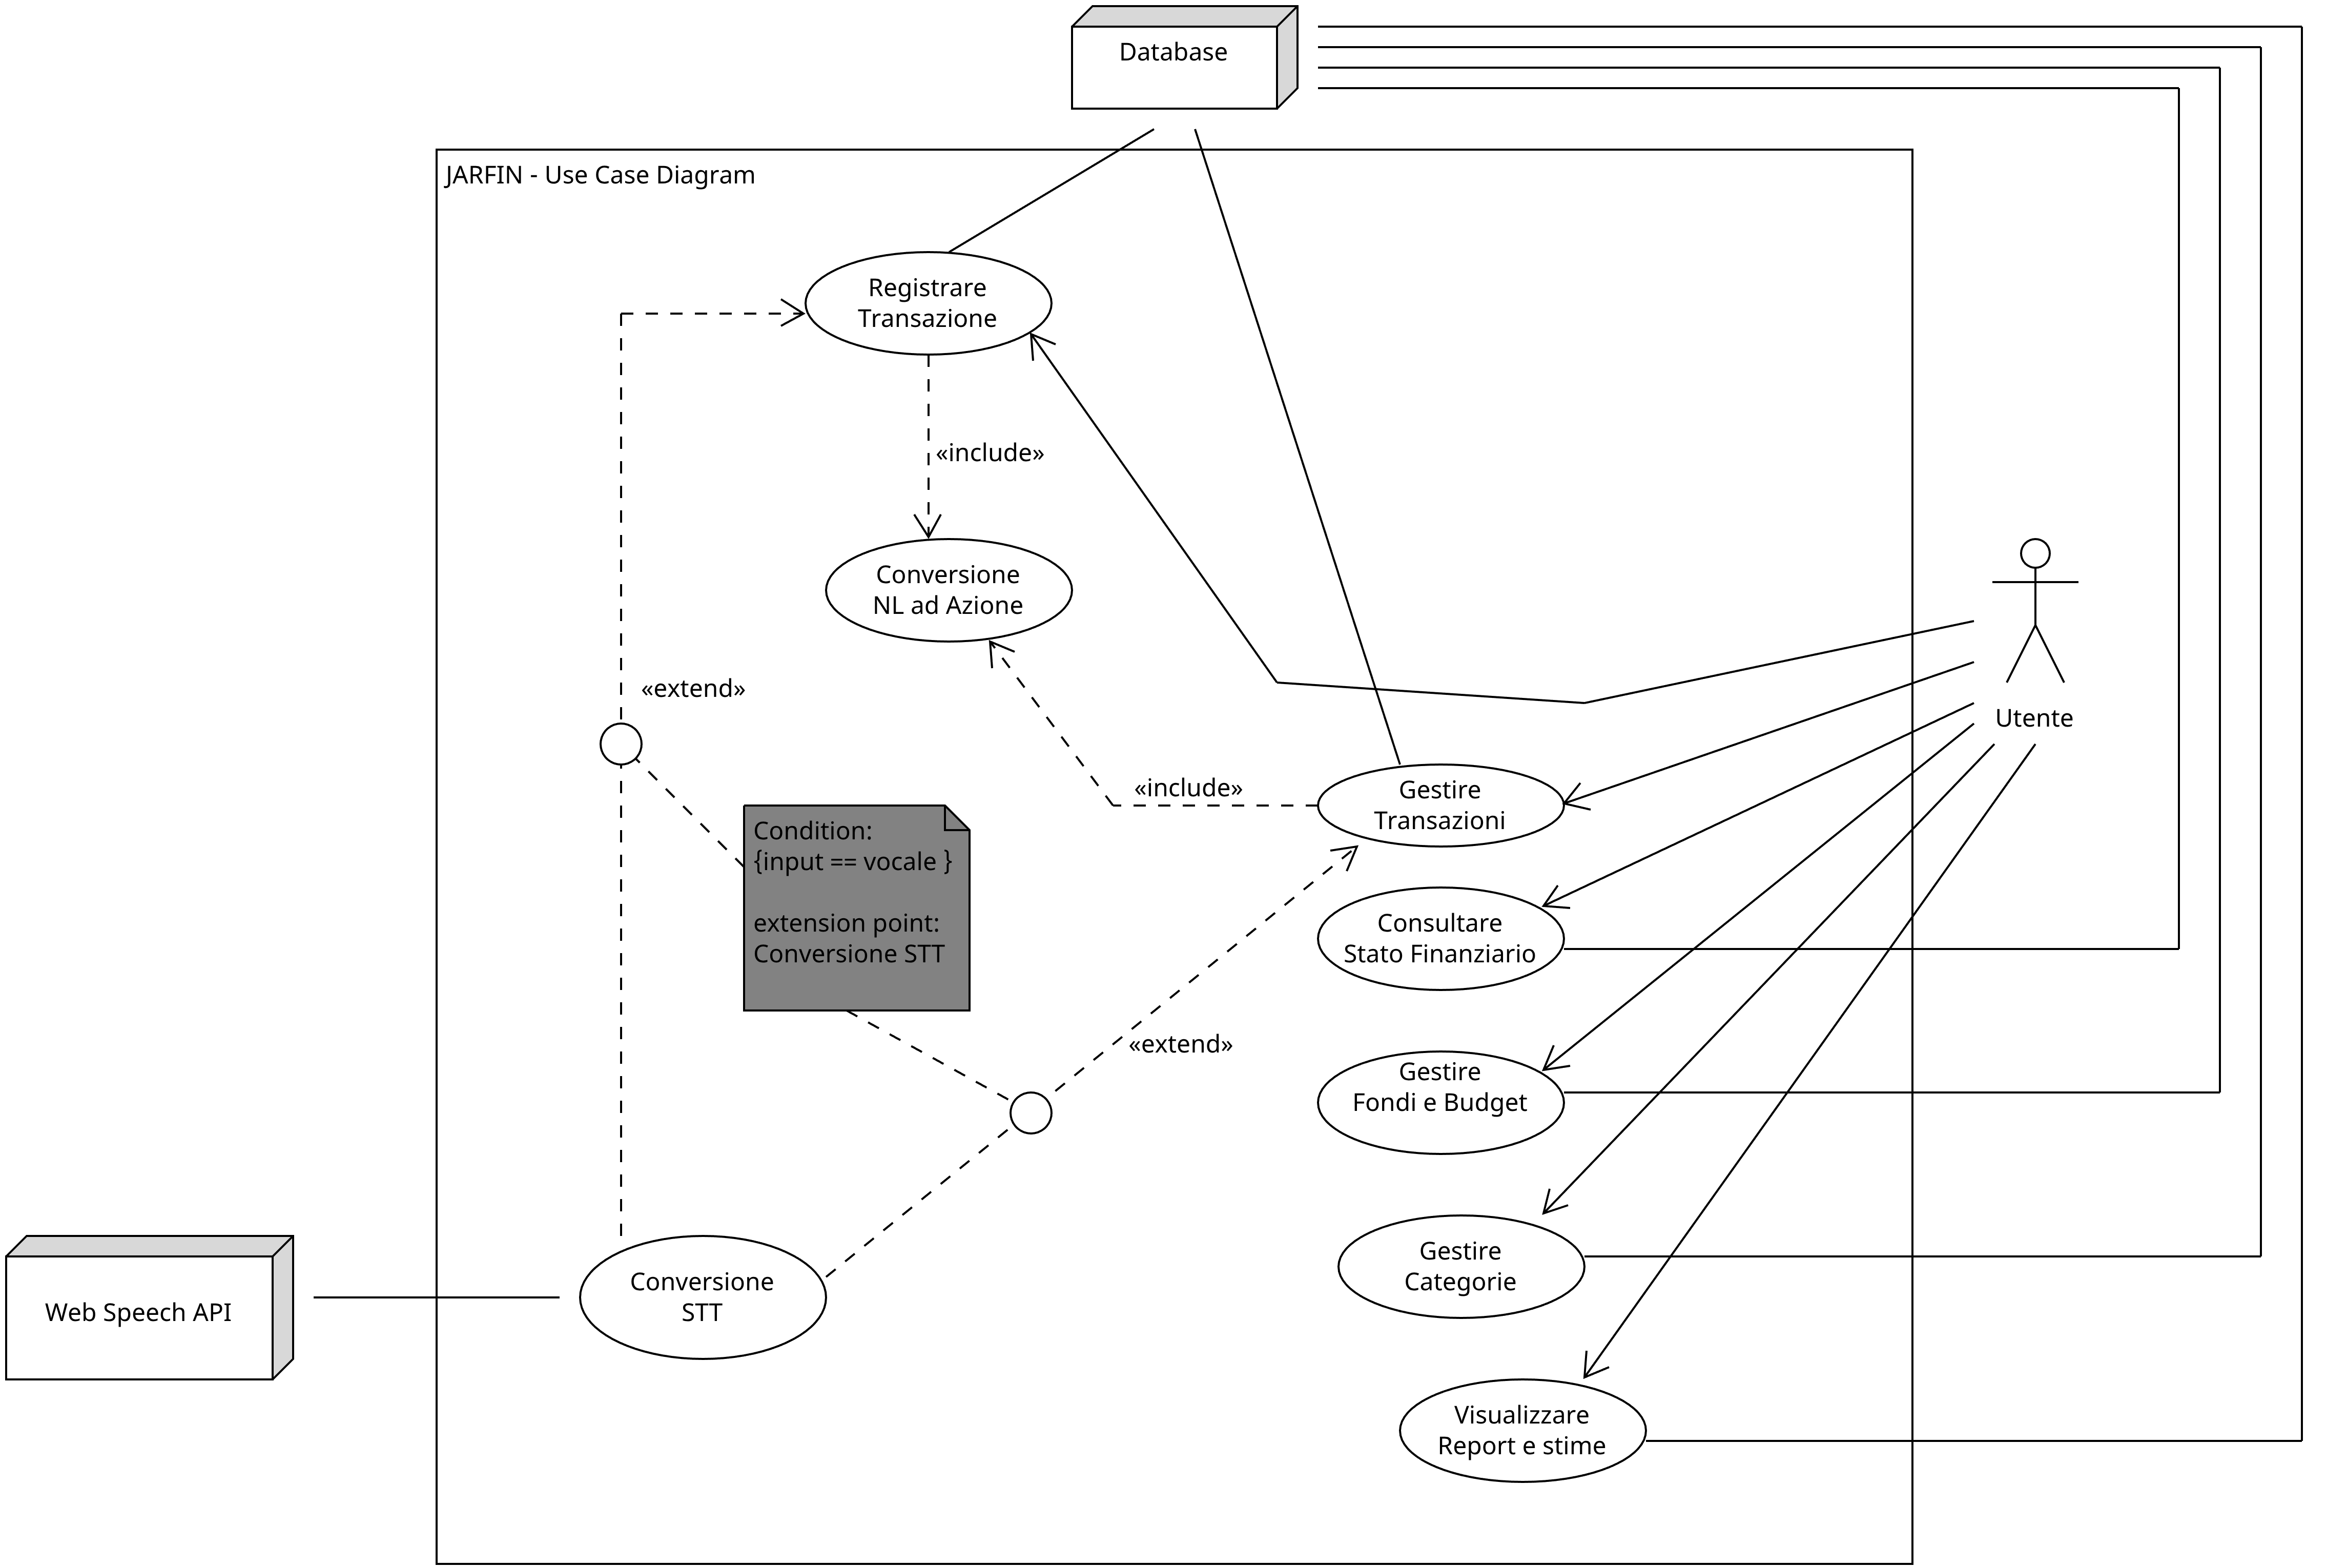
\includegraphics[width=1\textwidth]{../Iterazione_0/images/use_case_diagram.png}
    \caption{Diagramma dei casi d'uso (Vista degli Scenari).}
    \label{fig:use_case}
\end{figure}

\subsection{Attori}
Il diagramma identifica due tipologie di attori:
\begin{itemize}
    \item \textbf{Utente}: attore primario che interagisce con l'interfaccia web per la gestione delle proprie finanze.
    \item \textbf{Sistemi esterni}: attori secondari necessari al funzionamento del backend:
          \begin{itemize}
              \item \textbf{Cloud Speech-to-Text}: servizio invocato per la trascrizione dei comandi vocali;
              \item \textbf{Database}: sistema responsabile della persistenza fisica di tutte le entità (utenti, transazioni, categorie).
          \end{itemize}
\end{itemize}

\subsection{Descrizione dei Casi d'Uso}

Le funzionalità sono state raggruppate in tre macro-aree logiche per facilitarne la lettura e l'implementazione.



\subsubsection{Gestione Transazioni}
Rappresenta il nucleo operativo dell'applicazione (\textit{Core Domain}).
\begin{itemize}
    \item \textbf{Registrare Transazione}: permette l'inserimento di una nuova spesa o entrata.
          \begin{itemize}
              \item \textit{Inclusione («include»)}: include obbligatoriamente il caso d'uso \textbf{"Conversione NL ad Azione"}, poiché ogni input (testuale o vocale) deve essere processato dal parser NLU per estrarre i dati strutturati.
              \item \textit{Estensione («extend»)}: è esteso da \textbf{"Conversione STT"} se la condizione \texttt{input == vocale} è soddisfatta.
          \end{itemize}
    \item \textbf{Gestire Transazioni}: permette la modifica o l'eliminazione di movimenti esistenti.
          \begin{itemize}
              \item Anche questo caso d'uso include la logica di parsing NLU ed è esteso dalla conversione vocale, permettendo all'utente di modificare i dati tramite comandi vocali.
          \end{itemize}
\end{itemize}

\subsubsection{Analisi e Configurazione}
Riguarda le funzionalità di monitoraggio e organizzazione dei dati.
\begin{itemize}
    \item \textbf{Consultare Stato Finanziario}: visualizzazione immediata del saldo attuale.
    \item \textbf{Gestire Fondi e Budget}: definizione dei limiti di spesa mensili.
    \item \textbf{Gestire Categorie}: permette all'utente di creare, modificare o eliminare le categorie di spesa personalizzate (es. "Svago", "Casa").
    \item \textbf{Visualizzare Report e Stime}: generazione di grafici e proiezioni future basate sullo storico delle transazioni.
\end{itemize}

\newpage
\section{Vista logica – Class Diagram}

La vista logica (Figura \ref{fig:classdiagram}) illustra la struttura statica del sistema, evidenziando la suddivisione in microservizi e le relazioni tra le classi. Il diagramma riflette l'architettura modulare adottata, dove ogni componente ha responsabilità ben definite.

\begin{figure}[H]
    \centering
    \includegraphics[width=1\textwidth]{../Iterazione_0/images/class_diagram.png}
    \caption{Diagramma di classi (Vista Logica).}
    \label{fig:classdiagram}
\end{figure}

\subsection{Shared Kernel e Modello di Dominio}
La parte sinistra del diagramma definisce le entità core del sistema, che costituiscono il linguaggio comune tra i vari microservizi:
\begin{itemize}
    \item \textbf{\texttt{Transaction}}: Definita come una \textit{Abstract Class}, rappresenta l'entità fondamentale. Include i campi \texttt{id} (Long), \texttt{amount} (BigDecimal), \texttt{date} (LocalDate), \texttt{description}, \texttt{category} e \texttt{type}.
    \item \textbf{\texttt{Category}}: Entità dedicata alla classificazione delle operazioni (es. "Cibo", "Casa"). È legata a \texttt{Transaction} da una relazione di associazione "belongs to" con cardinalità $1$ a $0..n$.
    \item \textbf{\texttt{Budget}}: Classe utilizzata per monitorare le soglie di spesa. Presenta gli attributi \texttt{limitAmount}, \texttt{spentAmount} e un riferimento a un \texttt{Period}. È collegata alla classe \texttt{Category} con una relazione $1:1$.
    \item \textbf{\texttt{Period}}: Una classe di supporto che modella un intervallo temporale tramite \texttt{startDate} e \texttt{endDate} (Date). Questa entità è condivisa sia da \texttt{Budget} che dalla logica di \texttt{Report} per definire l'ambito temporale delle analisi.
\end{itemize}

\subsection{Microservizio Accounting}
Situato nella parte inferiore, implementa il classico pattern a tre livelli per la gestione dei dati finanziari:
\begin{itemize}
    \item \textbf{\texttt{TransactionController}}: espone gli endpoint REST per le operazioni CRUD.
    \item \textbf{\texttt{TransactionService}}: incapsula la logica di business e valida i dati in ingresso.
    \item \textbf{\texttt{TransactionRepository}}: interfaccia che estende \textit{Spring Data JPA}, gestendo l'accesso diretto al database.
\end{itemize}

\subsection{NLU Service (Natural Language Understanding)}
Il modulo gestisce l'interpretazione dei comandi vocali e testuali, evidenziando una struttura orientata al pattern matching e al processamento asincrono:
\begin{itemize}
    \item \textbf{\texttt{CommandController}}: Riceve i payload dalla WEB UI (endpoint \texttt{POST /process}) e coordina l'interazione tra il servizio NLU e il resto del sistema tramite \texttt{RestTemplate}.
    \item \textbf{\texttt{NaturalLanguageService}}: Il componente core che esegue il parsing del testo utilizzando pattern predefiniti (\texttt{NUMBER\_PATTERN}, \texttt{DELETE\_CMD}) e una \texttt{CATEGORY\_MAP} per estrarre i dati.
    \item \textbf{\texttt{ParsedTransaction}}: Un oggetto contenitore (DTO) che racchiude l'intento estratto, includendo il \texttt{CommandType} (CREATE, DELETE, UPDATE), l'importo, la categoria e la descrizione.
    \item \textbf{\texttt{SpeechToTextService}}: Definita come \textit{Interface}, rappresenta un'astrazione «future». Attualmente, la trascrizione avviene lato client tramite Web Speech API in \texttt{index.html}.
\end{itemize}

\subsection{Analytics Service}
Localizzato nel package dedicato, si occupa della generazione della reportistica finanziaria:
\begin{itemize}
    \item \textbf{\texttt{AnalyticsController}}: Espone l'endpoint \texttt{getReport()} che restituisce un oggetto di tipo \texttt{FinancialReportDTO}.
    \item \textbf{\texttt{AnalyticsService}}: Contiene la logica di business per aggregare i dati e invocare la creazione del \texttt{Report} tramite il metodo \texttt{generateReport()}.
    \item \textbf{\texttt{FinancialReportDTO}}: Struttura dati ottimizzata per il frontend che include i totali (\texttt{totExp}, \texttt{totInc}) e il dettaglio dei totali per categoria (\texttt{totByCategory}).
\end{itemize}

\subsection{Accounting Service}
Modulo preposto alla gestione della persistenza e della logica transazionale:
\begin{itemize}
    \item \textbf{\texttt{TransactionController}}: Punto di ingresso per la gestione delle transazioni (\texttt{createTransaction}, \texttt{getTransactions}).
    \item \textbf{\texttt{TransactionService}}: Implementa i metodi operativi come \texttt{addExp()} (aggiunta spesa) e \texttt{addInc()} (aggiunta entrata).
    \item \textbf{\texttt{TransactionRepository}}: Interfaccia per l'accesso ai dati, con metodi specifici come \texttt{saveTransaction()} e \texttt{findByPeriod()}.
\end{itemize}

\subsection{Orchestrazione e API Gateway}
L'architettura utilizza un \textbf{\texttt{APIGateway}} all'interno del package \texttt{API}:
\begin{itemize}
    \item \textbf{Routing}: Il Gateway funge da unico punto di accesso, esponendo metodi per l'autenticazione (\texttt{authUser}) e il routing delle richieste (\texttt{route}) verso i controller dei microservizi.
    \item \textbf{Dipendenze}: Le linee tratteggiate indicano una dipendenza d'uso verso \texttt{TransactionController}, \texttt{AnalyticsController} e \texttt{NaturalLanguageService}, confermando il suo ruolo di orchestratore del traffico.
\end{itemize}

\section{Vista di sviluppo – Component Diagram}

Il Diagramma dei Componenti (Figura \ref{fig:components}) illustra l'organizzazione del sistema JarFin [cite: 4] in moduli software distinti e le dipendenze che intercorrono tra di essi. Questa vista evidenzia una struttura a tre livelli (\textit{Layered Architecture}):

\begin{figure}[H]
    \centering
    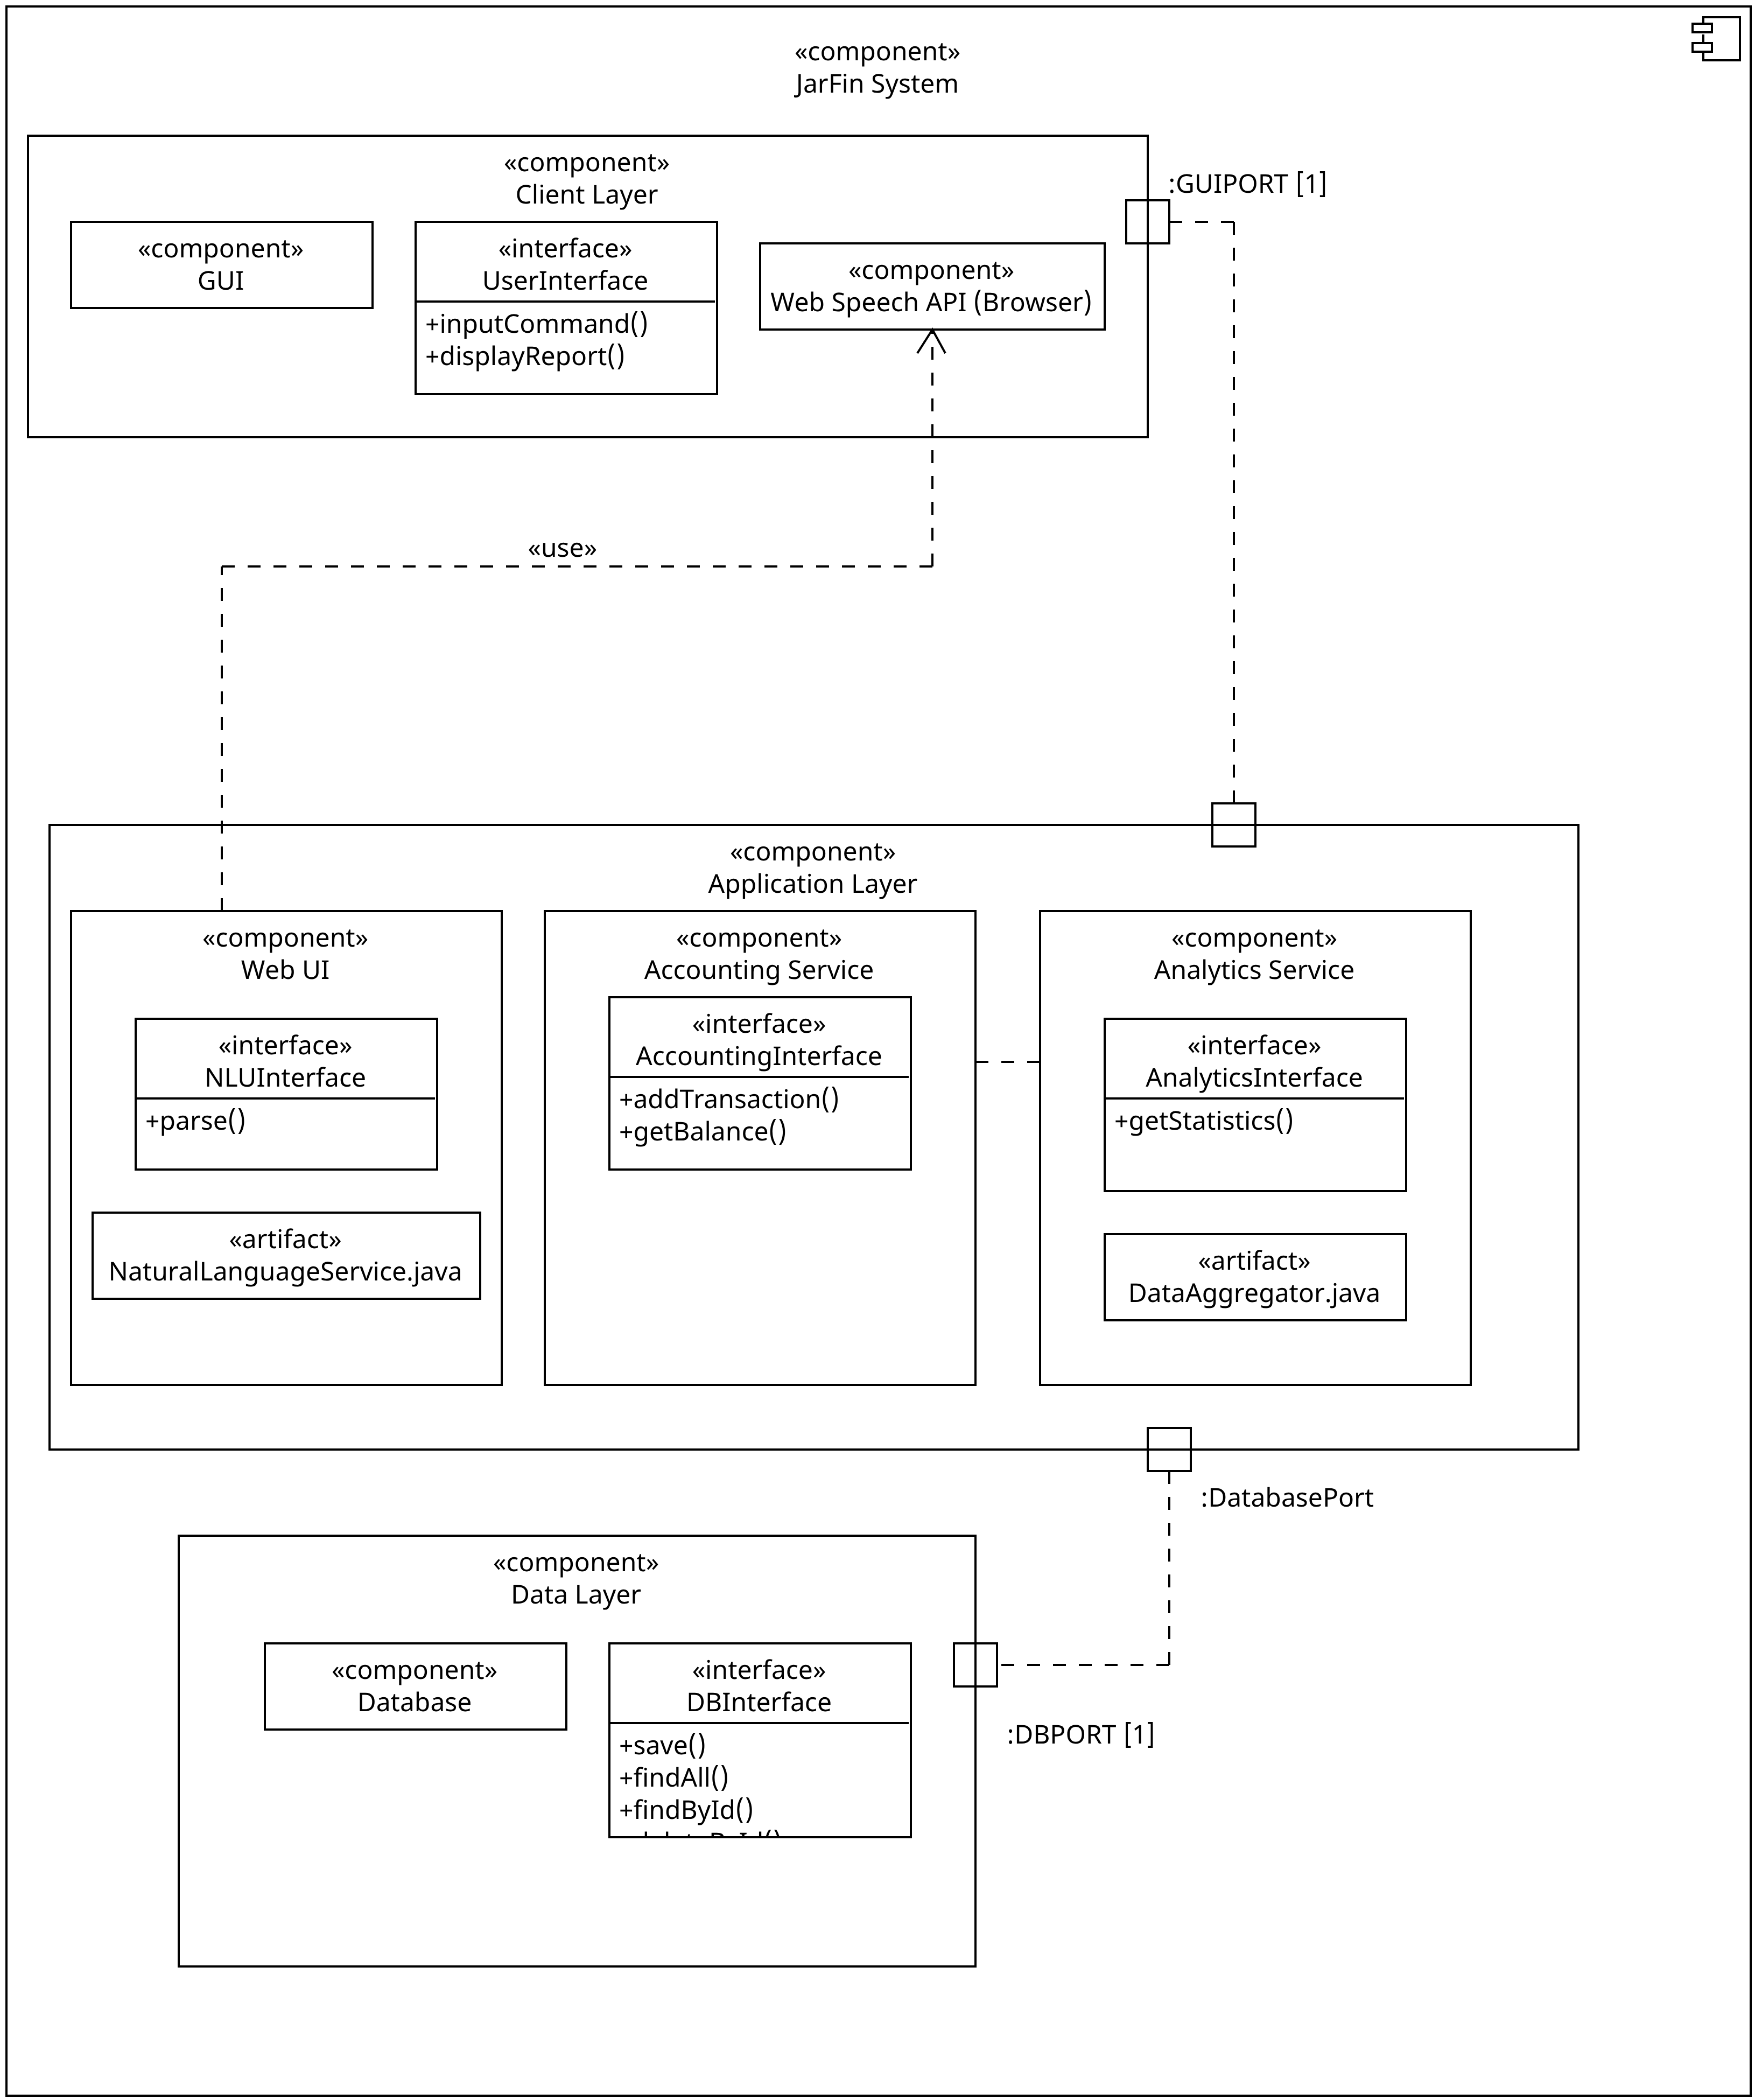
\includegraphics[width=0.78\textwidth]{../Iterazione_0/images/component_diagram.png}
    \caption{Diagramma dei componenti: architettura a livelli e interfacce esposte.}
    \label{fig:components}
\end{figure}

\subsection{Client Layer}
Il livello superiore rappresenta il frontend e i servizi di interazione immediata con l'utente:
\begin{itemize}
    \item \textbf{GUI}: Componente che gestisce la logica di visualizzazione, implementando l'interfaccia \texttt{UserInterface} con i metodi \texttt{inputCommand()} e \texttt{displayReport()}.
    \item \textbf{Web Speech API (Browser)}: Componente che fornisce le capacità di riconoscimento vocale integrate nel browser.
    \item \textbf{Porte}: La comunicazione verso i livelli sottostanti è veicolata tramite la \texttt{GUIPORT [1]}.
\end{itemize}

\subsection{Application Layer}
Il nucleo del sistema incapsula la logica di business ed è suddiviso in tre moduli principali che operano all'interno del componente \texttt{Web UI} e dei servizi backend:
\begin{itemize}
    \item \textbf{NLU Service}: Incapsula l'artefatto \texttt{NaturalLanguageService.java} e fornisce l'interfaccia \texttt{NLUInterface} per l'operazione di \texttt{parse()}.
    \item \textbf{Accounting Service}: Gestisce i flussi finanziari tramite l'interfaccia \texttt{AccountingInterface}, esponendo i metodi \texttt{addTransaction()} e \texttt{getBalance()}.
    \item \textbf{Analytics Service}: Utilizza l'artefatto \texttt{DataAggregator.java} per elaborare i dati tramite l'interfaccia \texttt{AnalyticsInterface} e il metodo \texttt{getStatistics()}[cite: 5, 3].
\end{itemize}

\subsection{Data Layer}
Il livello di persistenza è isolato dal resto dell'applicazione per garantire l'indipendenza dallo storage:
\begin{itemize}
    \item \textbf{Database}: Componente responsabile dell'archiviazione dei dati.
    \item \textbf{DBInterface}: L'interfaccia di accesso ai dati che astrae le operazioni CRUD fondamentali: \texttt{save()}, \texttt{findAll()}, \texttt{findById()} e \texttt{deleteById()}.
    \item \textbf{Porte}: Riceve le richieste dal livello applicativo sulla porta \texttt{DBPORT [1]} attraverso una connessione verso la \texttt{DatabasePort}.
\end{itemize}

\subsection{Dipendenze e Relazioni}
\begin{itemize}
    \item \textbf{Relazione di Uso}: Il componente \texttt{Web UI} all'interno dell'Application Layer presenta una dipendenza \texttt{«use»} verso la \texttt{Web Speech API} del Client Layer per le funzionalità STT.
    \item \textbf{Integrazione}: I componenti \texttt{Accounting Service} e \texttt{Analytics Service} appaiono interconnessi per permettere l'aggregazione dei dati transazionali ai fini statistici.
\end{itemize}


\section{Vista di processo – Sequence Diagram}

La vista di processo descrive la dinamica temporale delle interazioni tra gli attori e i componenti del sistema JarFin durante l'esecuzione di un comando. Il diagramma (Figura \ref{fig:sequence}) illustra il flusso completo, dalla ricezione dell'input alla persistenza dei dati e alla generazione del feedback.

\begin{figure}[H]
    \centering
    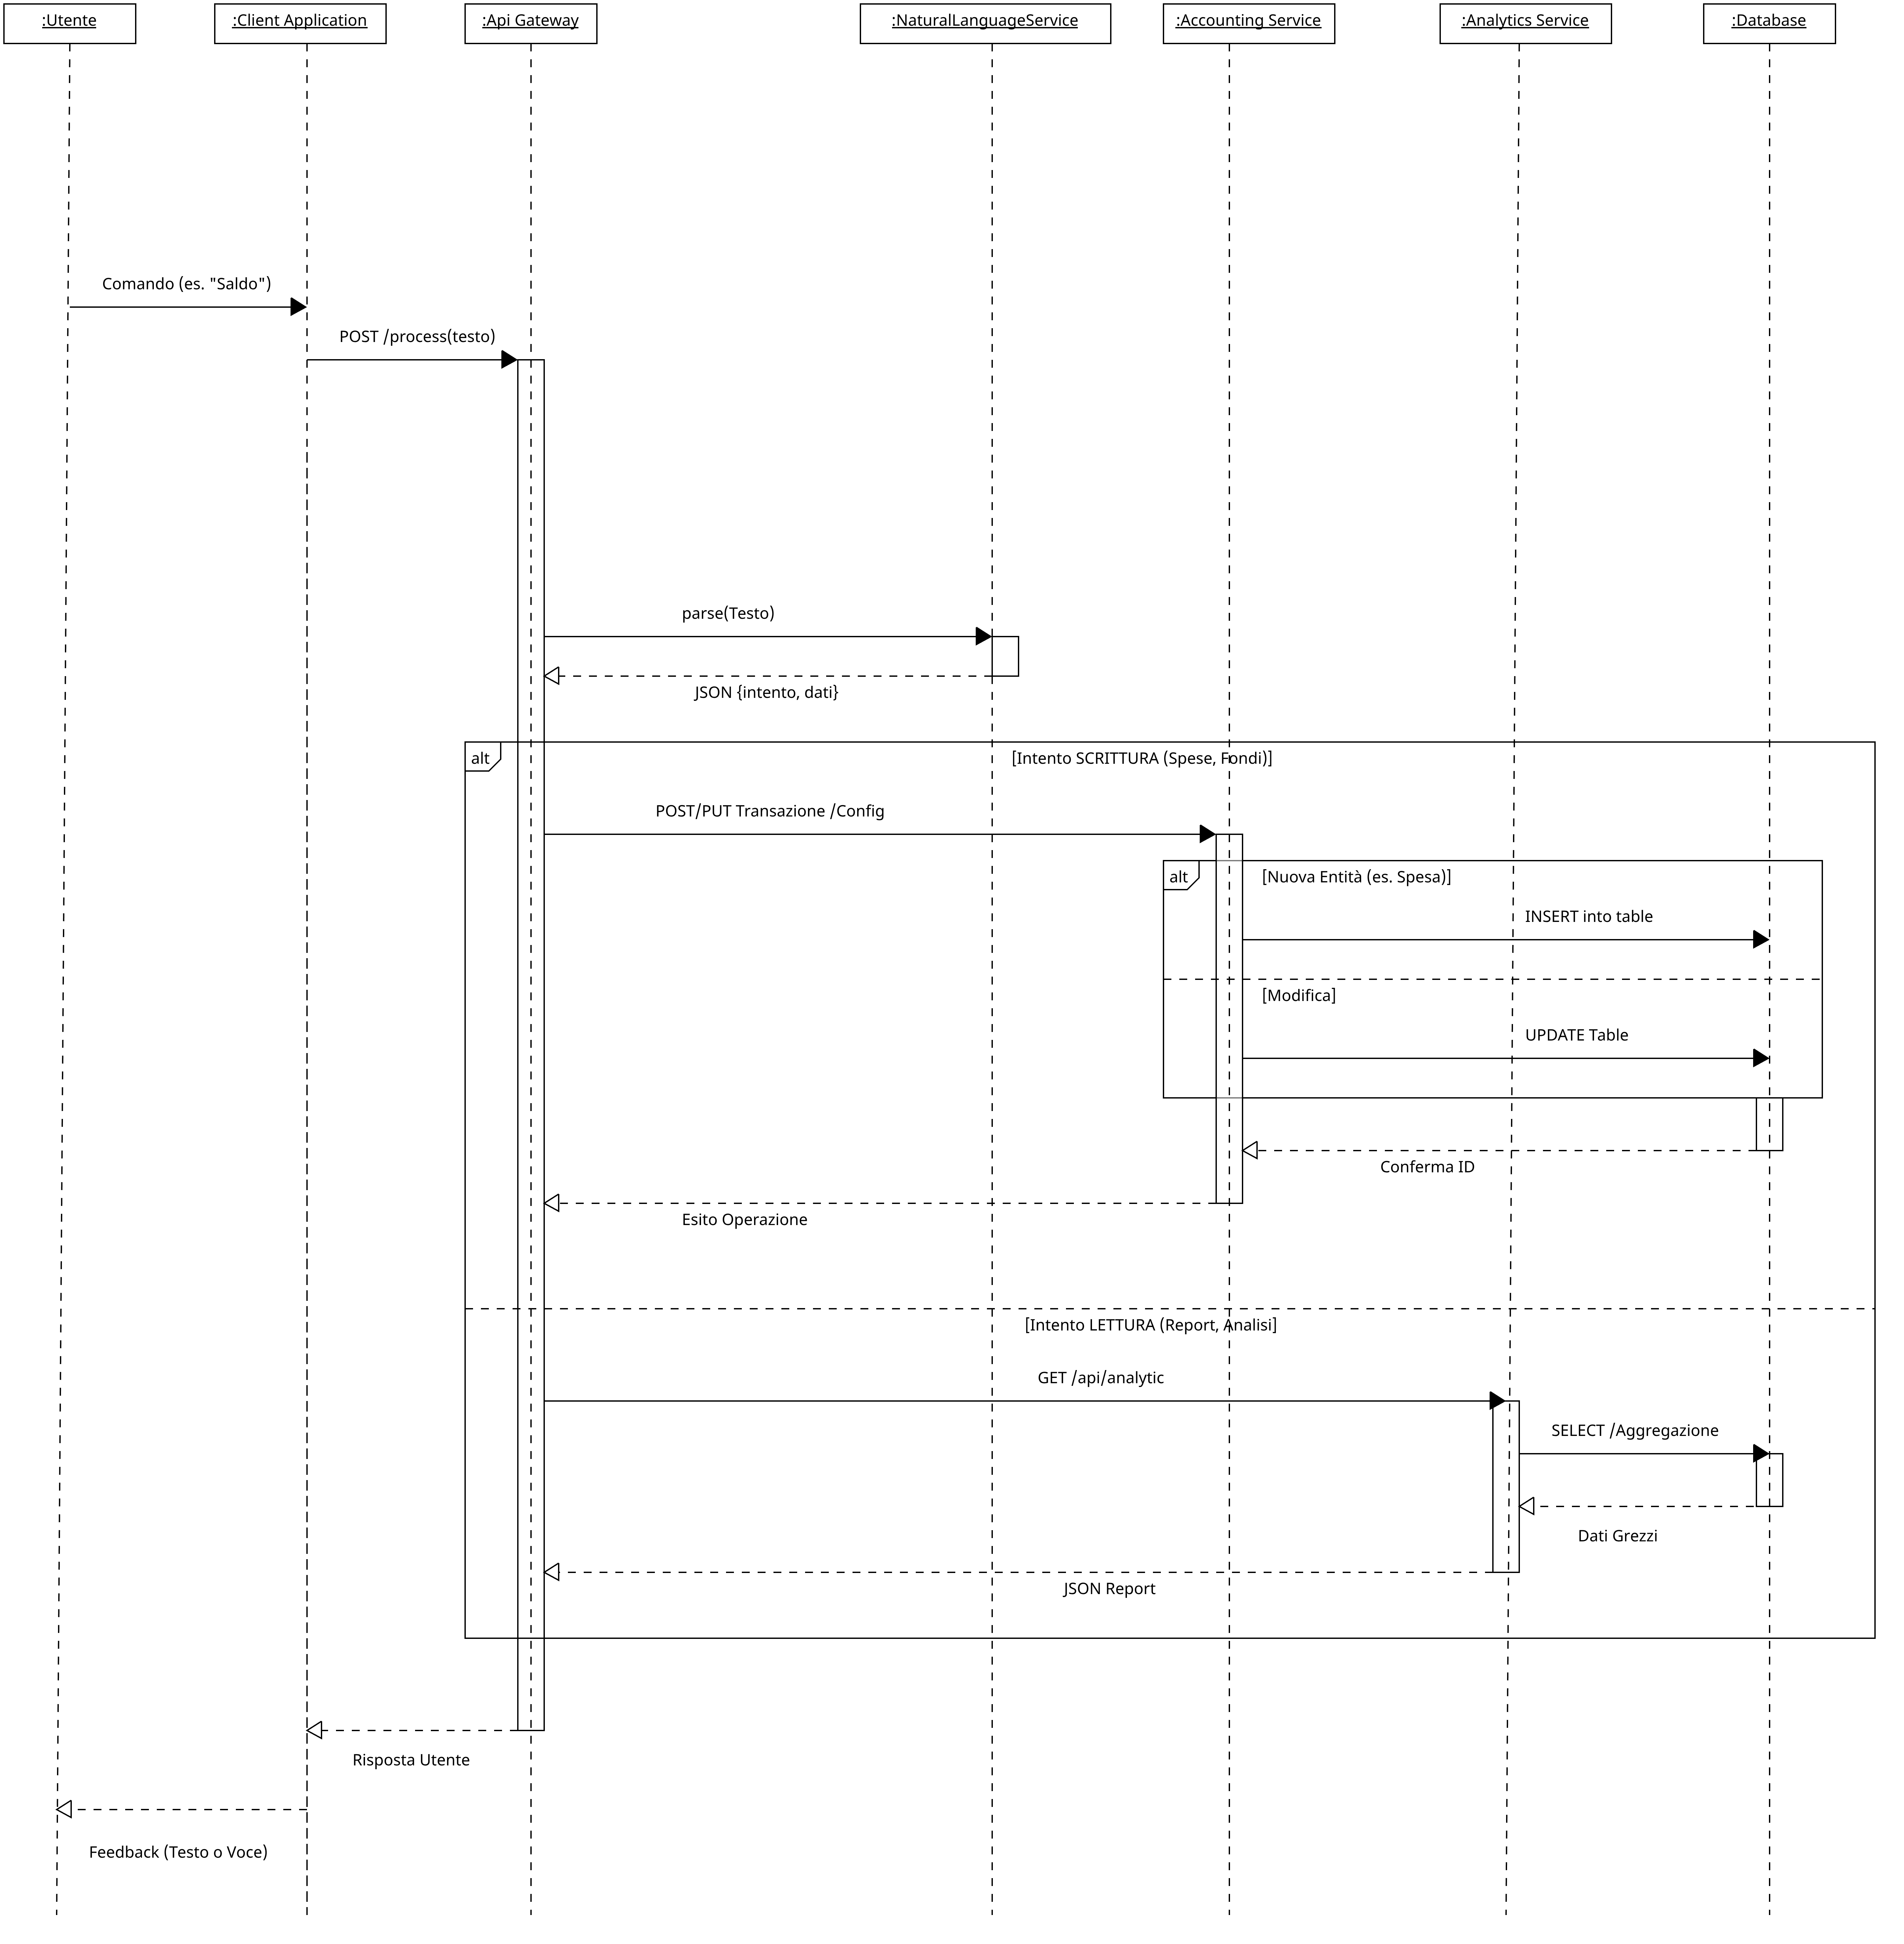
\includegraphics[width=0.8\textwidth]{../Iterazione_0/images/sequence_diagram.png}
    \caption{Diagramma di sequenza: autenticazione, gestione comandi e routing.}
    \label{fig:sequence}
\end{figure}

\newpage
\subsection{Fase 1: Input e Pre-elaborazione}
Il flusso ha inizio con l'interazione dell'utente verso l'applicazione client:
\begin{enumerate}
    \item \textbf{Invio Comando}: L'utente invia un comando (es. "Saldo") alla \texttt{Client Application} [cite: 15].
    \item \textbf{Inoltro Richiesta}: La \texttt{Client Application} effettua una chiamata \texttt{POST /process(testo)} verso l'\texttt{Api Gateway}.
    \item \textbf{Analisi Semantica}: L'Gateway invoca il metodo \texttt{parse(Testo)} del \texttt{NaturalLanguageService}. Il servizio restituisce un oggetto \texttt{JSON \{intento, dati\}} che identifica l'azione richiesta.
\end{enumerate}

\subsection{Fase 2: Elaborazione Condizionale (Frammento \texttt{alt})}
In base all'intento estratto dal servizio NLU, il sistema segue due percorsi logici distinti:

\begin{itemize}
    \item \textbf{Intento SCRITTURA (Spese, Fondi)}: 
          L'Gateway inoltra una richiesta \texttt{POST/PUT} all'\textbf{Accounting Service}. All'interno di questo ramo, un ulteriore frammento \texttt{alt} distingue l'operazione sul \texttt{Database}:
          \begin{itemize}
              \item \textit{Nuova Entità}: Viene eseguita una \texttt{INSERT into table} (es. per una nuova Spesa)[cite: 14, 16].
              \item \textit{Modifica}: Viene eseguita una \texttt{UPDATE Table}.
          \end{itemize}
          Il Database restituisce una \texttt{Conferma ID} all'Accounting Service, che a sua volta comunica l'\texttt{Esito Operazione} all'Gateway.

    \item \textbf{Intento LETTURA (Report, Analisi)}: 
          L'Gateway invoca l'\textbf{Analytics Service} tramite \texttt{GET /api/analytics/report(Filtri)}. Il servizio esegue una query di \texttt{SELECT / Aggregazione} sul \texttt{Database}, riceve i \texttt{Dati Grezzi} e li trasforma in un \texttt{JSON Report} per l'Gateway.
\end{itemize}

\subsection{Fase 3: Feedback Finale}
Una volta completata l'elaborazione nei microservizi, il ciclo si conclude con la notifica all'utente:
\begin{enumerate}
    \item L'\texttt{Api Gateway} invia la \texttt{Risposta Utente} alla \texttt{Client Application}.
    \item L'applicazione mostra il \texttt{Feedback} finale (sotto forma di testo o voce) all'utente.
\end{enumerate}

\section{Vista fisica – Deployment Diagram}

Il Diagramma di Deployment (Figura \ref{fig:deployment}) illustra la distribuzione fisica del sistema JarFin, mappando gli artefatti software sui nodi hardware e descrivendo i protocolli di comunicazione utilizzati.

\begin{figure}[H]
    \centering
    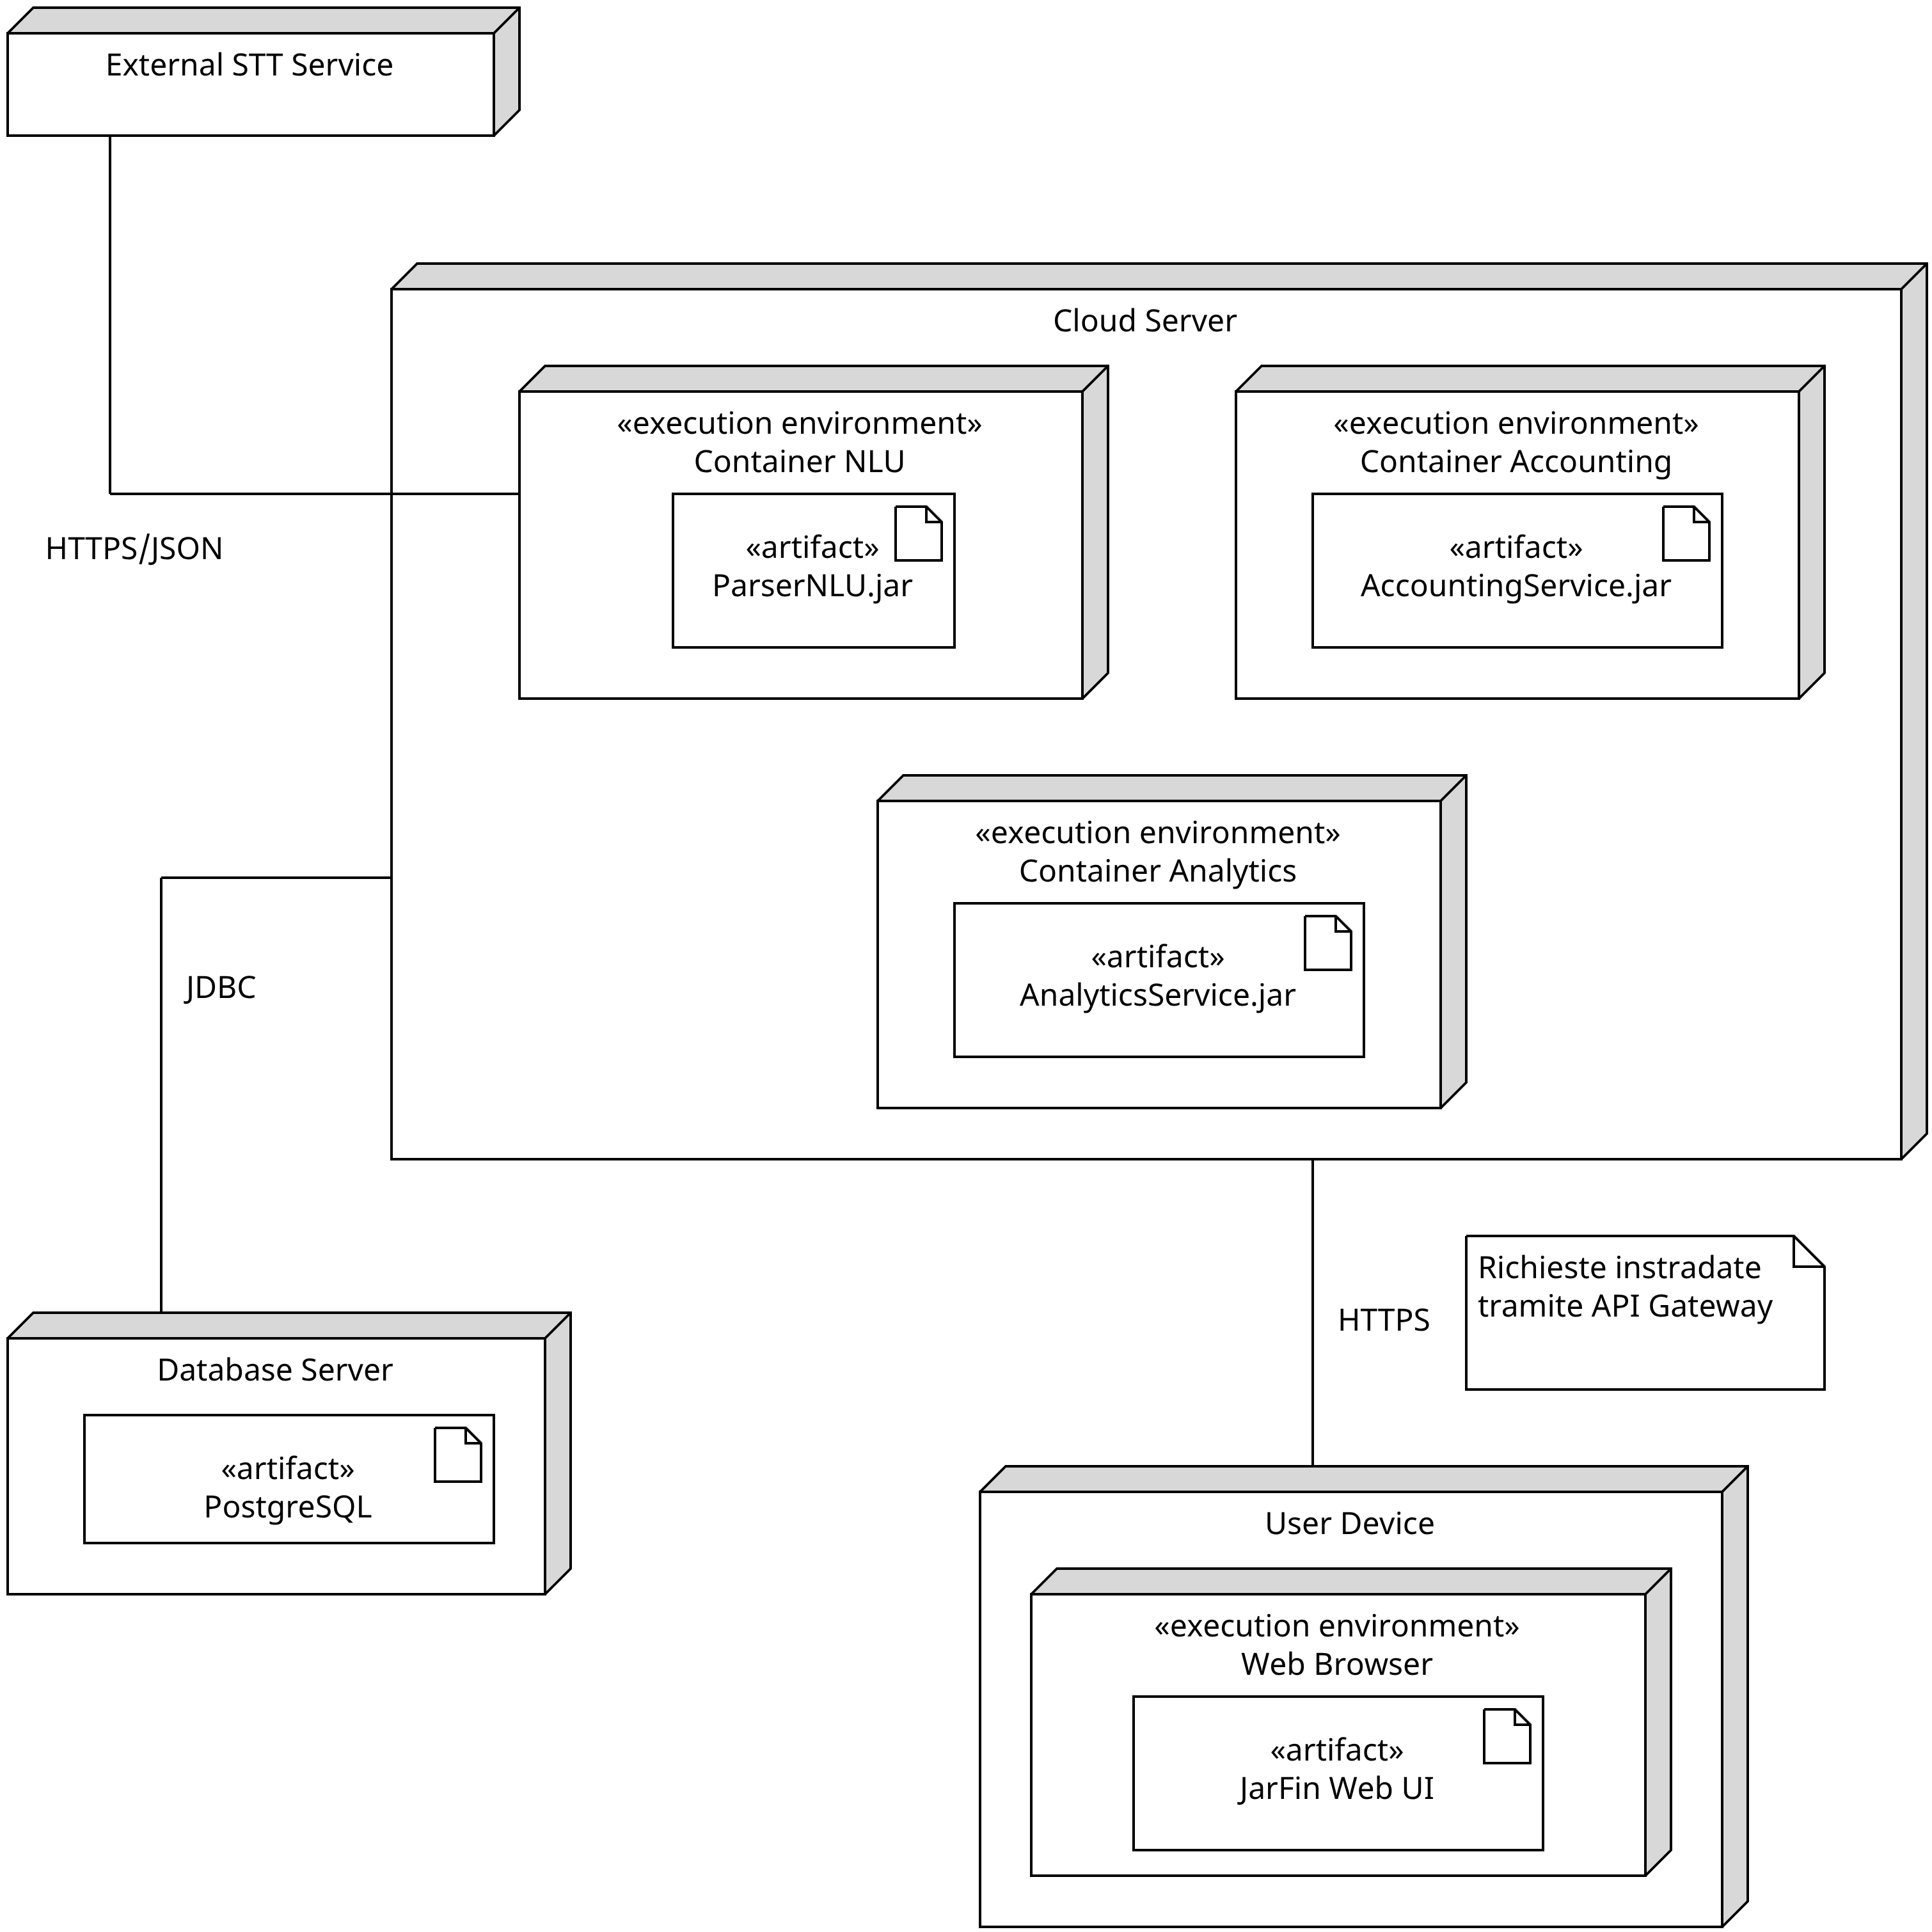
\includegraphics[width=0.8\textwidth]{../Iterazione_0/images/deployment_diagram.png}
    \caption{Diagramma di deployment: nodi fisici, container e protocolli di rete.}
    \label{fig:deployment}
\end{figure}

\subsection{Architettura dei Nodi e Ambienti}
Il sistema è distribuito su infrastrutture distinte che separano il frontend, la logica applicativa e la persistenza:

\begin{itemize}
    \item \textbf{User Device}: Rappresenta il dispositivo terminale dell'utente. Ospita l'ambiente di esecuzione \textbf{Web Browser} [cite: 31], all'interno del quale viene eseguito l'artefatto \textbf{\texttt{jarfin-web-ui.jar}}. In questo nodo è presente anche il supporto alle \textbf{Web Speech API} per il riconoscimento vocale direttamente lato client.

    \item \textbf{Cloud Server}: Il nodo centrale che ospita i microservizi. È suddiviso in ambienti di esecuzione containerizzati per garantire l'isolamento:
          \begin{itemize}
              \item \textbf{Container Accounting}: Esegue l'artefatto \texttt{AccountingService.jar}[cite: 28, 30].
              \item \textbf{Analytics Service Container}: Esegue l'artefatto \texttt{AnalyticsService.jar}[cite: 28, 30].
              \item \textbf{Esecuzione NLU}: All'interno del server viene eseguito l'artefatto \texttt{ParserNLU.jar} per l'elaborazione del linguaggio naturale.
          \end{itemize}

    \item \textbf{Database Server}: Un nodo dedicato che ospita il DBMS \textbf{PostgreSQL}, garantendo che la persistenza dei dati sia fisicamente separata dalla logica di business per ottimizzare sicurezza e performance.
\end{itemize}

\subsection{Protocolli di Comunicazione}
Le interconnessioni tra i vari nodi utilizzano protocolli standard per lo scambio di dati:

\begin{itemize}
    \item \textbf{User Device $\xrightarrow{HTTPS/JSON}$ Cloud Server}: La comunicazione tra il browser dell'utente e il server applicativo avviene tramite il protocollo \textbf{HTTPS}. I dati vengono scambiati in formato \textbf{JSON}, permettendo al client di inviare comandi e ricevere report o conferme.

    \item \textbf{Cloud Server $\xrightarrow{JDBC}$ Database Server}: L'accesso ai dati da parte dei microservizi (in particolare il servizio Accounting) avviene tramite una connessione \textbf{JDBC} verso l'istanza di PostgreSQL.

    \item \textbf{Integrazione Locale}: A differenza di implementazioni puramente cloud, il diagramma evidenzia che la componente di trascrizione vocale (\textbf{Web Speech API}) risiede nello \textit{User Device}, riducendo la necessità di inviare flussi audio grezzi verso nodi esterni per il solo STT.
\end{itemize}

\newpage
\section{Conclusioni dell'Iterazione 0}

L'attività di analisi e progettazione ha prodotto un'architettura solida, modulare e documentata. L'adozione del modello 4+1 ha permesso di affrontare la complessità del sistema distribuito, definendo chiaramente le responsabilità di ogni componente prima dell'inizio della fase di codifica (Iterazione 1).

% 4. Iterazione 1 (Accounting Service, Docker, Testing)
\chapter{Iterazione 1: Implementazione dell'Accounting Service}
\label{chap:iterazione1}

\section{Introduzione e Obiettivi dell'Iterazione}

L'Iterazione 1 del progetto \textit{JarFin} ha rappresentato la fase fondativa dello sviluppo, dedicata alla progettazione e alla realizzazione del microservizio \textbf{Accounting Service}. Questo componente costituisce il nucleo operativo dell'intera architettura, essendo responsabile della gestione autoritativa delle transazioni finanziarie (registrazione, consultazione, modifica e cancellazione).

L'obiettivo primario di questa fase non si è limitato alla semplice implementazione delle funzionalità CRUD (\textit{Create, Read, Update, Delete}), ma ha riguardato la costruzione di un'infrastruttura software solida, basata sui principi della \textit{Clean Architecture} e pronta per supportare la scalabilità futura.
Le sfide principali affrontate hanno riguardato:

\begin{itemize}
    \item \textbf{Infrastruttura}: Configurazione di un ambiente di sviluppo containerizzato e riproducibile tramite Docker.
    \item \textbf{Persistenza}: Gestione rigorosa dei dati su un RDBMS relazionale (PostgreSQL).
    \item \textbf{Architettura}: Definizione di pattern per la validazione, la gestione centralizzata degli errori e il disaccoppiamento dei dati (DTO/Mapper).
    \item \textbf{Qualità}: Garanzia della robustezza del codice tramite una strategia di testing ibrida (Unitari e di Integrazione).
\end{itemize}

\section{Stack Tecnologico e Configurazione}

Il microservizio è stato sviluppato adottando uno stack tecnologico moderno, scelto per garantire robustezza e facilità di manutenzione:

\begin{itemize}
    \item \textbf{Java 21}: Utilizzato come linguaggio di programmazione, sfruttando le ultime funzionalità LTS (\textit{Long Term Support}) per massimizzare performance e sicurezza.
    \item \textbf{Spring Boot 3.2.0}: Framework di riferimento per lo sviluppo di microservizi in ambiente Java. Ha permesso di abbattere i tempi di configurazione (\textit{Convention over Configuration}) fornendo un server web integrato (Tomcat) e la gestione automatica delle dipendenze.
    \item \textbf{Spring Data JPA / Hibernate}: Per la gestione della persistenza tramite ORM (\textit{Object-Relational Mapping}), astraendo la complessità delle query SQL dirette.
    \item \textbf{PostgreSQL 16}: Scelto come RDBMS per la sua affidabilità, il supporto alle transazioni ACID e la capacità di gestire carichi di lavoro complessi.
    \item \textbf{Docker \& Docker Compose}: Per l'orchestrazione dell'ambiente di sviluppo e la containerizzazione del database.
    \item \textbf{Lombok}: Libreria utilizzata per ridurre il codice "boilerplate" (getter, setter, costruttori), migliorando la leggibilità delle classi.
    \item \textbf{Maven}: Per la gestione del ciclo di vita del software e delle dipendenze, come definito nel file \texttt{pom.xml}.
\end{itemize}

\section{Orchestrazione dell'Ambiente (Docker Compose)}

Una delle prime decisioni architetturali è stata quella di disaccoppiare l'applicazione dall'installazione locale del database. Per garantire che l'ambiente di sviluppo fosse deterministico e identico per ogni sviluppatore, si è optato per la virtualizzazione tramite \textbf{Docker}.

Il file \texttt{docker-compose.yml} definisce il servizio di database e le sue configurazioni:

\bigskip

\begin{lstlisting}[language=yaml, label={lst:dockercompose}]
services:
  db:
    image: postgres:15
    container_name: jarfin_db
    environment:
      POSTGRES_USER: ${DB_USER:-postgres}
      POSTGRES_PASSWORD: ${DB_PASSWORD:-password_segreta}
      POSTGRES_DB: jarfin_db
    ports:
      - "5432:5432"
    volumes:
      - postgres_data:/var/lib/postgresql/data

volumes:
  postgres_data:
\end{lstlisting}

\subsection{Analisi delle Scelte Implementative}
\begin{itemize}
    \item \textbf{Persistenza dei Dati}: L'uso di un volume nominato (\texttt{postgres\_data}) garantisce la persistenza dei dati anche in caso di arresto o rimozione dei container, evitando la perdita di informazioni tra le sessioni di sviluppo.
    \item \textbf{Sicurezza delle Credenziali}: Le credenziali di accesso non sono rigidamente fissate nel codice. La configurazione supporta l'iniezione tramite variabili d'ambiente (\texttt{\$\{DB\_PASSWORD\}}), con valori di default visibili solo per facilitare la revisione accademica. Questo approccio predispone il sistema per pipeline CI/CD sicure.
    \item \textbf{Networking}: Il database è esposto sulla porta 5432, permettendo connessioni sia dall'applicazione Spring Boot che da tool di amministrazione esterni (es. DBeaver/pgAdmin).
\end{itemize}

L'applicazione Spring Boot si connette al container in questione tramite il file \texttt{application.properties}, configurato per aggiornare automaticamente lo schema del database all'avvio (\texttt{spring.jpa.hibernate.ddl-auto=update}), accelerando notevolmente la fase di prototipazione.

\section{Architettura Software e Design Patterns}

Il microservizio implementa un'architettura a strati rigorosa (\textit{Layered Architecture}) per garantire la separazione delle responsabilità (\textit{Separation of Concerns}).
Il flusso dei dati attraversa i seguenti layer, in ordine:

\begin{itemize}
  \item \textbf{Controller (API)}: espone gli endpoint REST e gestisce le richieste HTTP;
  \item \textbf{Mapper / DTO}: converte i dati tra il modello di dominio e il contratto API;
  \item \textbf{Service (Business Logic)}: incapsula la logica applicativa;
  \item \textbf{Repository (Data Access)}: gestisce l’accesso e la persistenza dei dati.
\end{itemize}

\subsection{Modellazione del Dominio: La scelta di BigDecimal}
L'entità \texttt{Transaction} rappresenta il concetto centrale del dominio. Durante la modellazione, è stata posta particolare attenzione al tipo di dato per l'attributo \texttt{amount} (importo).

L'uso di tipi primitivi a virgola mobile come \texttt{double} o \texttt{float} è stato scartato a causa dell'imprecisione intrinseca nella rappresentazione binaria dei decimali (standard IEEE 754), che può portare a errori di arrotondamento inaccettabili in ambito finanziario.
È stato quindi adottato \texttt{java.math.BigDecimal}, che garantisce una precisione arbitraria e operazioni aritmetiche esatte.

\bigskip

\begin{lstlisting}[language=Java, label={lst:transactionentity}]
@Entity
@Table(name = "transactions")
@Getter @Setter @NoArgsConstructor
public class Transaction {
    @Id
    @GeneratedValue(strategy = GenerationType.IDENTITY)
    private Long id;

    @Column(nullable = false, precision = 19, scale = 4)
    private BigDecimal amount; // Precisione finanziaria garantita

    @Column(nullable = false)
    private LocalDate date;

    @Enumerated(EnumType.STRING)
    @Column(nullable = false)
    private TransactionType type; // INCOME o EXPENSE
    
    // ... altri campi (description, category)
}
\end{lstlisting}

Inoltre, per evitare problemi noti con i proxy di Hibernate, i metodi \texttt{equals()} e \texttt{hashCode()} sono stati implementati manualmente basandosi strettamente sull'identificatore univoco (\texttt{id}) dell'entità.

\subsection{Pattern DTO e Mapper}
Per disaccoppiare il modello di persistenza (Entity) dal contratto esposto all'esterno (API), è stato implementato il pattern DTO (Data Transfer Object).

\begin{itemize}
    \item \textbf{\texttt{TransactionRequest}}: Utilizzato per l'inserimento dati. Include annotazioni di Jakarta Validation (\texttt{@NotNull}, \texttt{@DecimalMin}, \texttt{@NotBlank}) per garantire che i dati in ingresso siano validi prima ancora di raggiungere la logica di business.
    \item \textbf{\texttt{TransactionResponse}}: Utilizzato per la risposta. Filtra eventuali dati tecnici non necessari al client.
\end{itemize}

La conversione tra Entity e DTO è centralizzata nella classe \texttt{TransactionMapper}, mantenendo il Controller e il Service puliti da logiche di trasformazione dei dati.

\section{Logica di Business e Gestione Errori}

\subsection{Service Layer}
La classe \texttt{TransactionService} incapsula la logica core. Un aspetto rilevante è l'uso dell'annotazione \texttt{@Transactional} sui metodi di modifica, che garantisce l'atomicità delle operazioni sul database: o l'operazione ha successo completamente, o viene eseguito un rollback.
Inoltre, è stato introdotto un sistema di logging (\texttt{@Slf4j}) per tracciare le operazioni critiche, fondamentale per il debugging in un ambiente distribuito.

\subsection{Gestione Centralizzata delle Eccezioni}
Invece di disseminare blocchi \texttt{try-catch} nel codice, è stato implementato un Global Exception Handler utilizzando \texttt{@RestControllerAdvice}.
Questo componente intercetta le eccezioni a livello globale e le trasforma in risposte JSON strutturate con i corretti codici di errore HTTP.

\bigskip

\begin{lstlisting}[language=Java, label={lst:globalhandler}]
@RestControllerAdvice
public class GlobalExceptionHandler {

    // Gestione 404 Not Found
    @ExceptionHandler(EntityNotFoundException.class)
    public ResponseEntity<String> handleNotFound(EntityNotFoundException ex) {
        return ResponseEntity.status(HttpStatus.NOT_FOUND).body(ex.getMessage());
    }

    // Gestione 400 Bad Request (Errori di Validazione)
    @ExceptionHandler(MethodArgumentNotValidException.class)
    public ResponseEntity<Map<String, String>> handleValidationErrors(
            MethodArgumentNotValidException ex) {
        Map<String, String> errors = new HashMap<>();
        ex.getBindingResult().getFieldErrors().forEach(error -> 
            errors.put(error.getField(), error.getDefaultMessage()));
        return ResponseEntity.badRequest().body(errors);
    }
}
\end{lstlisting}

Questo approccio migliora drasticamente l'usabilità dell'API: se un client invia un importo negativo, riceverà un errore 400 chiaro e dettagliato invece di un generico errore 500.

\section{Esposizione API: TransactionController}

Il \texttt{TransactionController} espone le funzionalità tramite endpoint RESTful standard. È stata posta particolare cura nel rispetto della semantica HTTP.
Il metodo \texttt{create}, in particolare, implementa il livello 2 del modello di maturità di Richardson (HTTP Verbs), restituendo l'header \texttt{Location} con l'URI della risorsa appena creata.

\bigskip

\begin{lstlisting}[language=Java, label={lst:createcontroller}]
@PostMapping
public ResponseEntity<TransactionResponse> create(@Valid @RequestBody TransactionRequest request) {
    Transaction entity = mapper.toEntity(request);
    Transaction saved = service.saveTransaction(entity);
    
    // Costruzione dinamica dell'URI della risorsa
    URI location = ServletUriComponentsBuilder.fromCurrentRequest()
            .path("/{id}")
            .buildAndExpand(saved.getId())
            .toUri();

    return ResponseEntity.created(location)
                         .body(mapper.toResponse(saved));
}
\end{lstlisting}

\section{Testing e Validazione}

La qualità del software sviluppato è stata verificata attraverso una strategia di testing su due livelli: automatizzato e manuale.

\subsection{Unit Testing (JUnit 5 \& Mockito)}
Sono stati sviluppati test unitari isolati per il Service e il Controller. L'uso di Mockito ha permesso di simulare il comportamento del database (`mocking`), verificando la logica di business e la corretta generazione delle risposte HTTP senza dipendenze esterne.
La Figura \ref{fig:junit} mostra l'esecuzione positiva della suite di test nell'ambiente di sviluppo.

\begin{figure}[H]
    \centering
    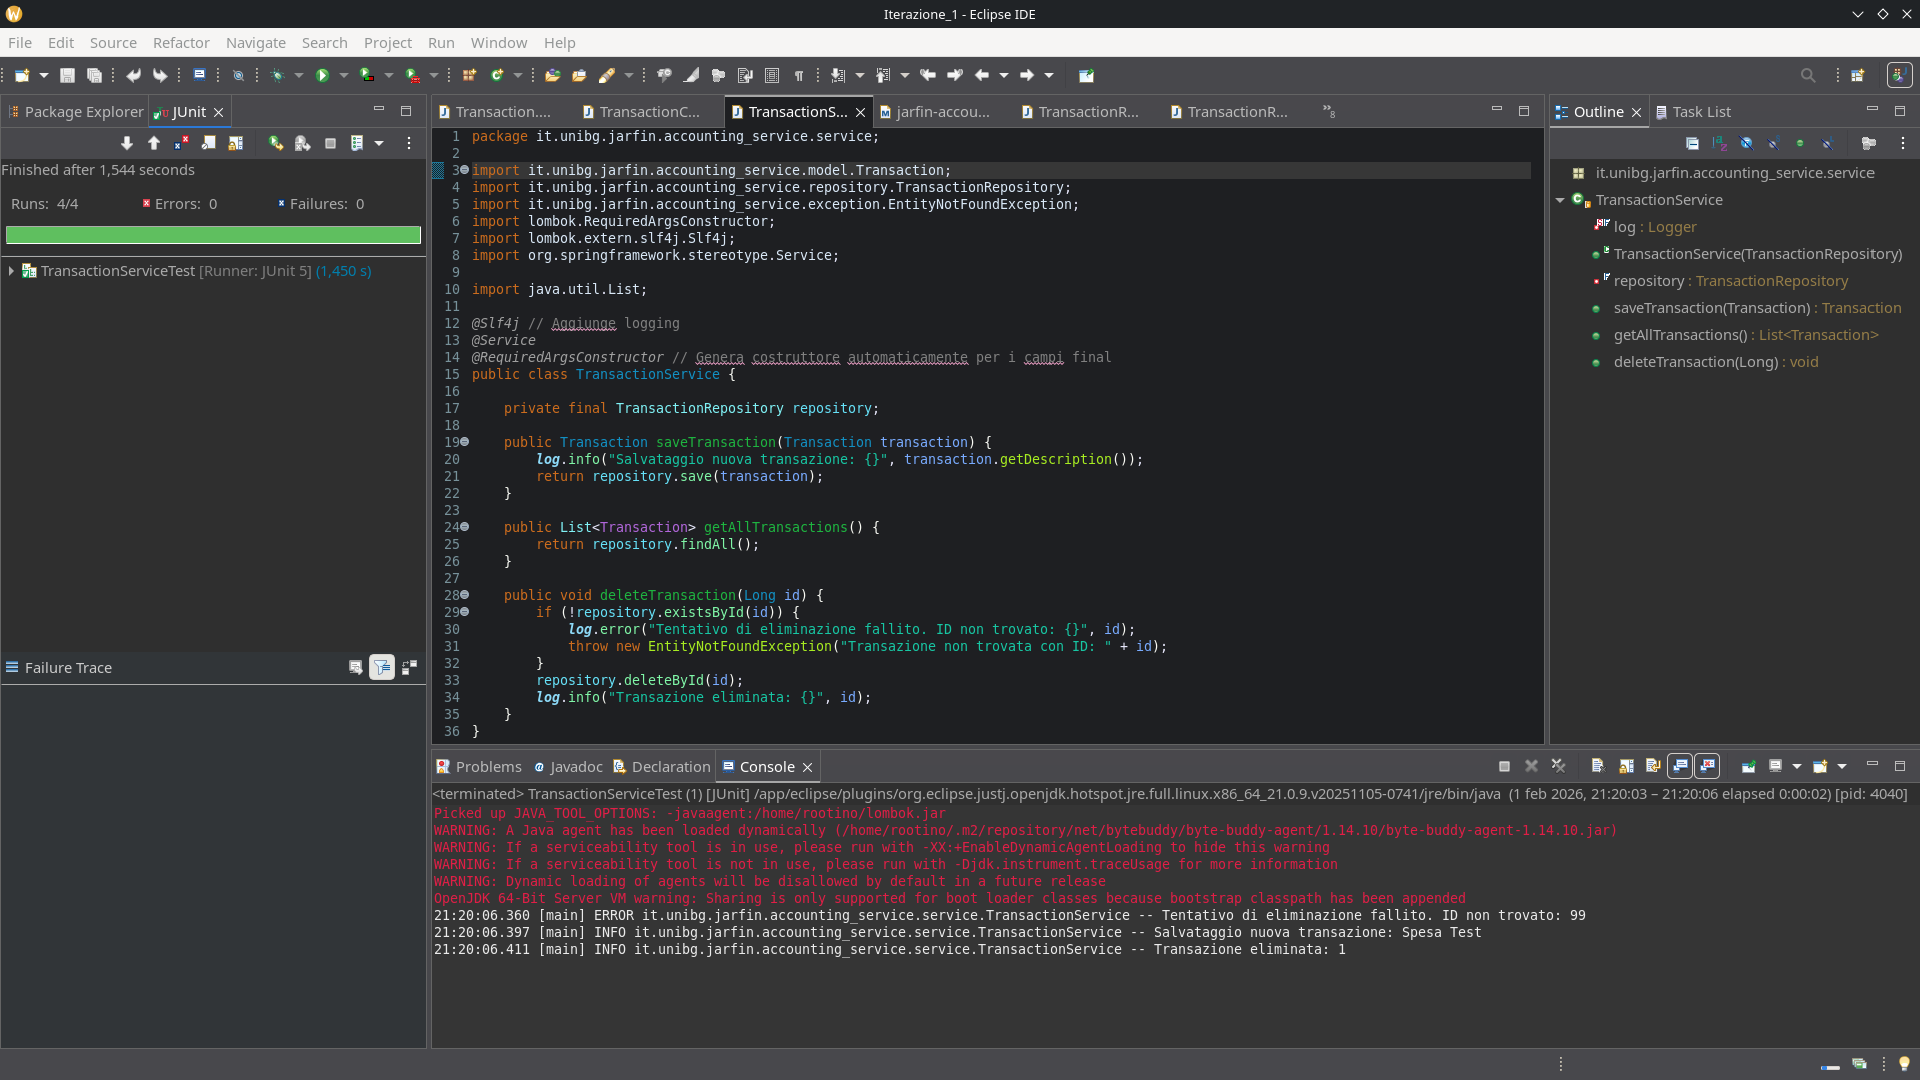
\includegraphics[width=0.9\textwidth]{../Iterazione_1/images/JUnit.png}
    \caption{Suite di test unitari completata con successo su TransactionService.java}
    \label{fig:junit}
\end{figure}

\subsection{Integration Testing (Postman)}
Per validare l'intero stack (Controller + Service + DB + Docker), sono stati eseguiti test manuali \textit{End-to-End} tramite Postman.

\textbf{1. Creazione Risorsa (Happy Path)}
Una richiesta \texttt{POST} valida (Figura \ref{fig:post_ok}) restituisce status \texttt{201 Created} e il JSON della transazione salvata, confermando il corretto funzionamento della catena di persistenza.
\begin{figure}[H]
    \centering
    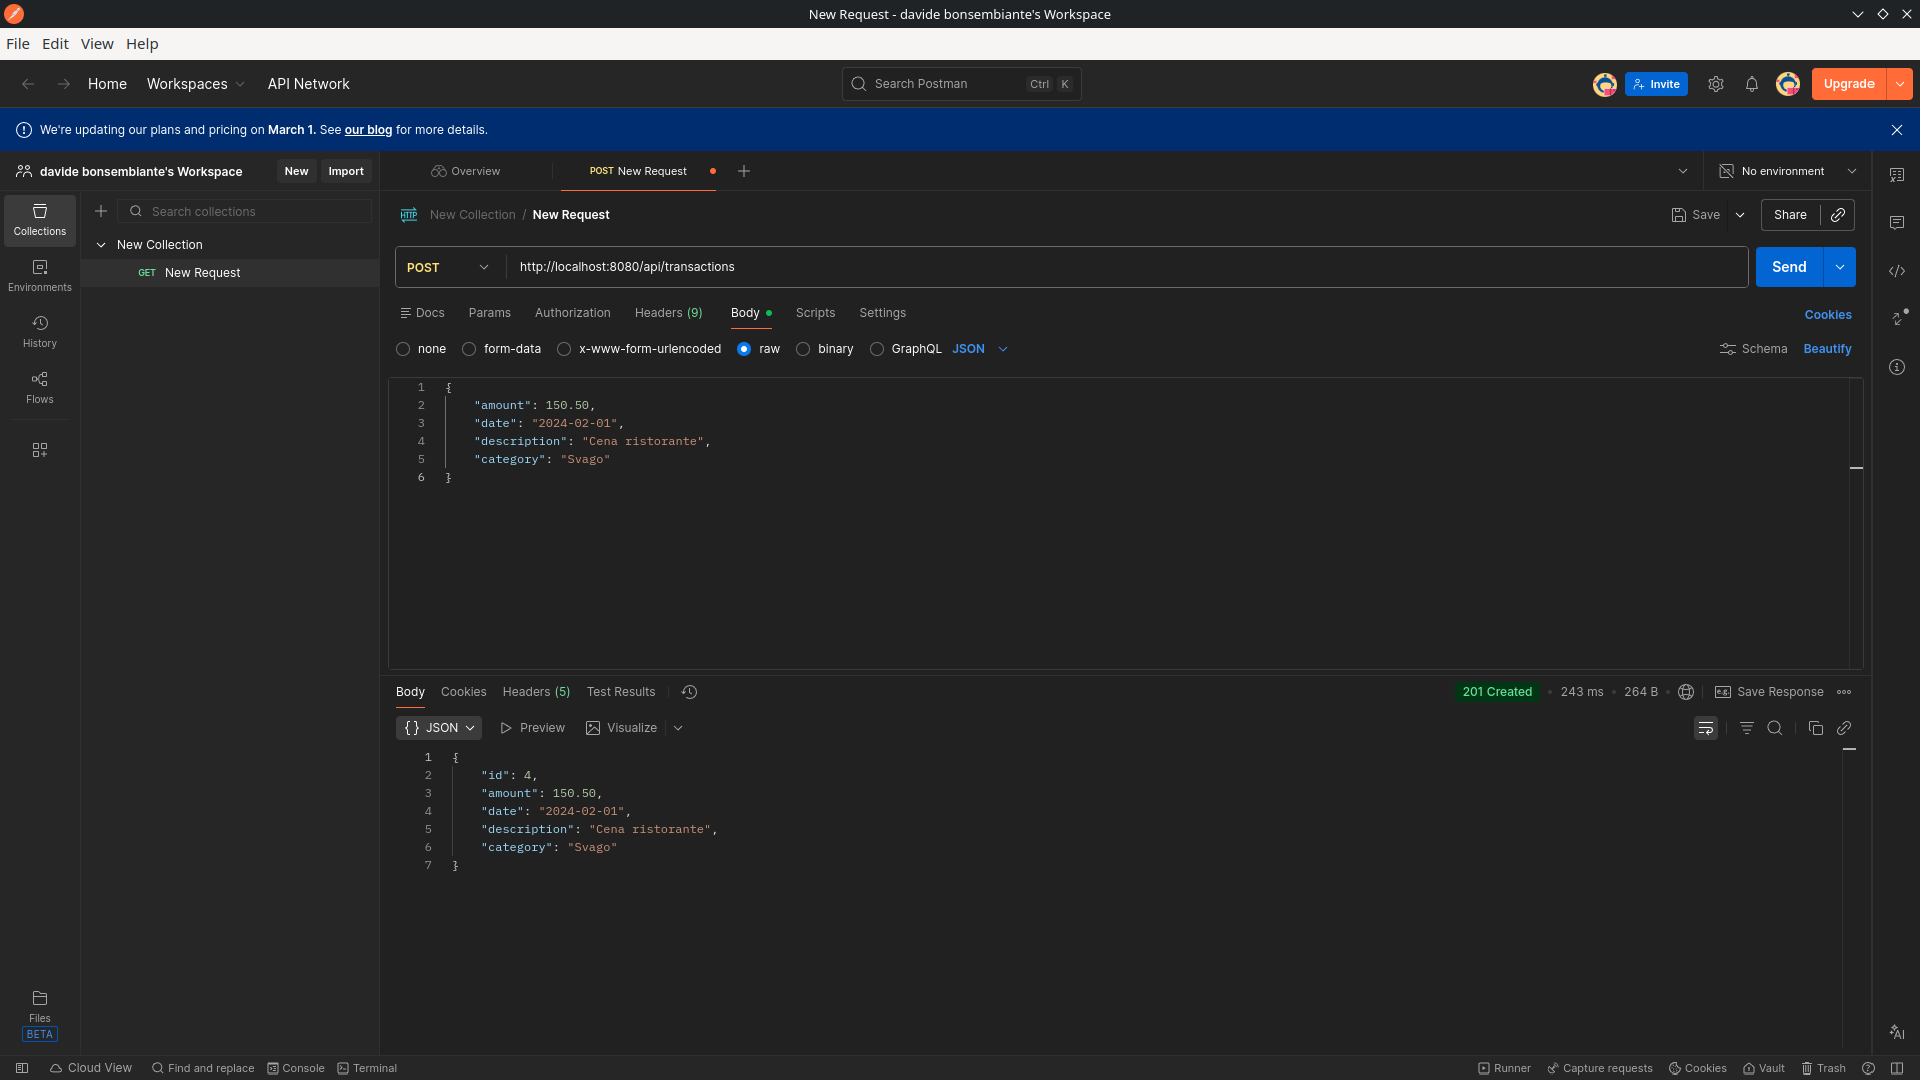
\includegraphics[width=1\textwidth]{../Iterazione_1/images/postman_post.png}
    \caption{Creazione di una transazione con successo (Status 201).}
    \label{fig:post_ok}
\end{figure}

\textbf{2. Recupero Dati}
La richiesta \texttt{GET} (Figura \ref{fig:get_ok}) conferma che i dati sono stati persistiti correttamente sul database PostgreSQL containerizzato.
\begin{figure}[H]
    \centering
    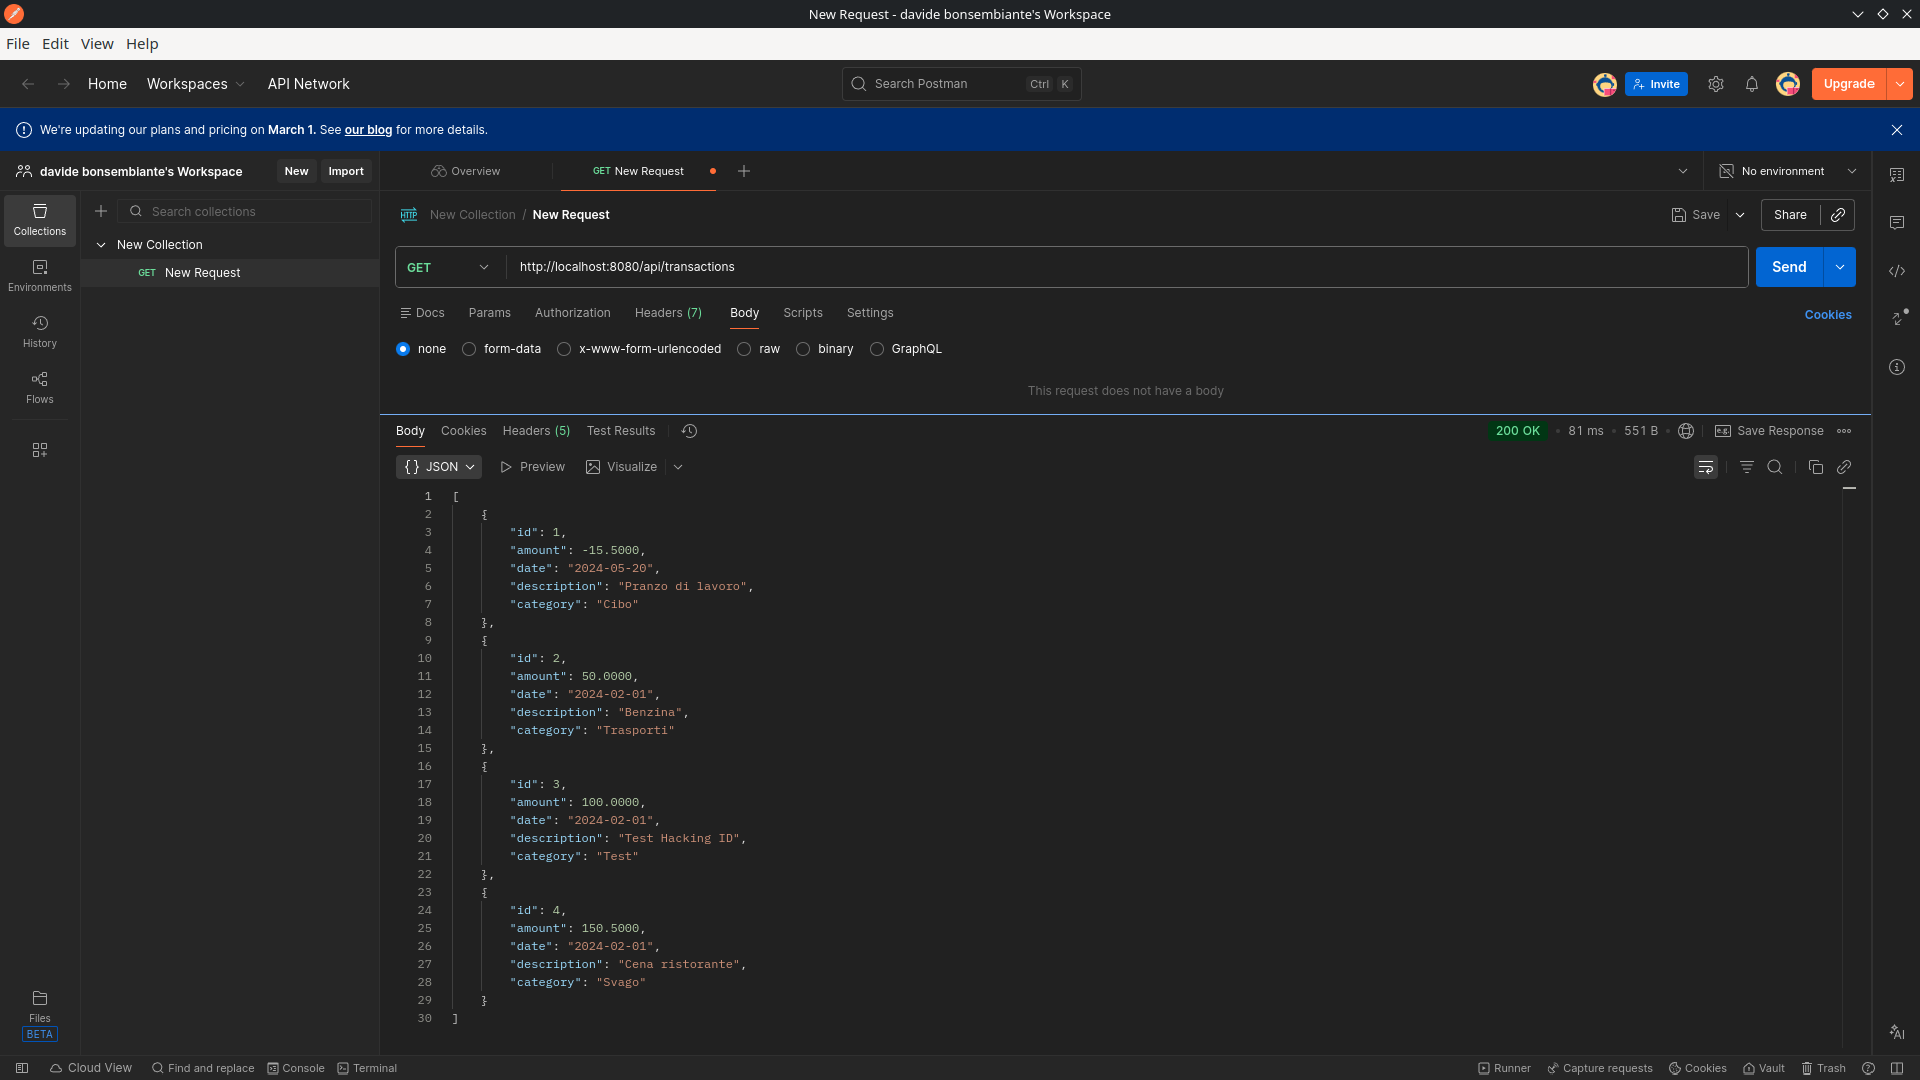
\includegraphics[width=1\textwidth]{../Iterazione_1/images/postman_get.png}
    \caption{Recupero della lista delle transazioni (Status 200).}
    \label{fig:get_ok}
\end{figure}

\textbf{3. Validazione Input (Error Handling)}
Inviando un payload con dati non validi (es. importo negativo), il sistema attiva il \texttt{GlobalExceptionHandler} (Figura \ref{fig:post_bad}), restituendo un \texttt{400 Bad Request} con i dettagli dell'errore.
\begin{figure}[H]
    \centering
    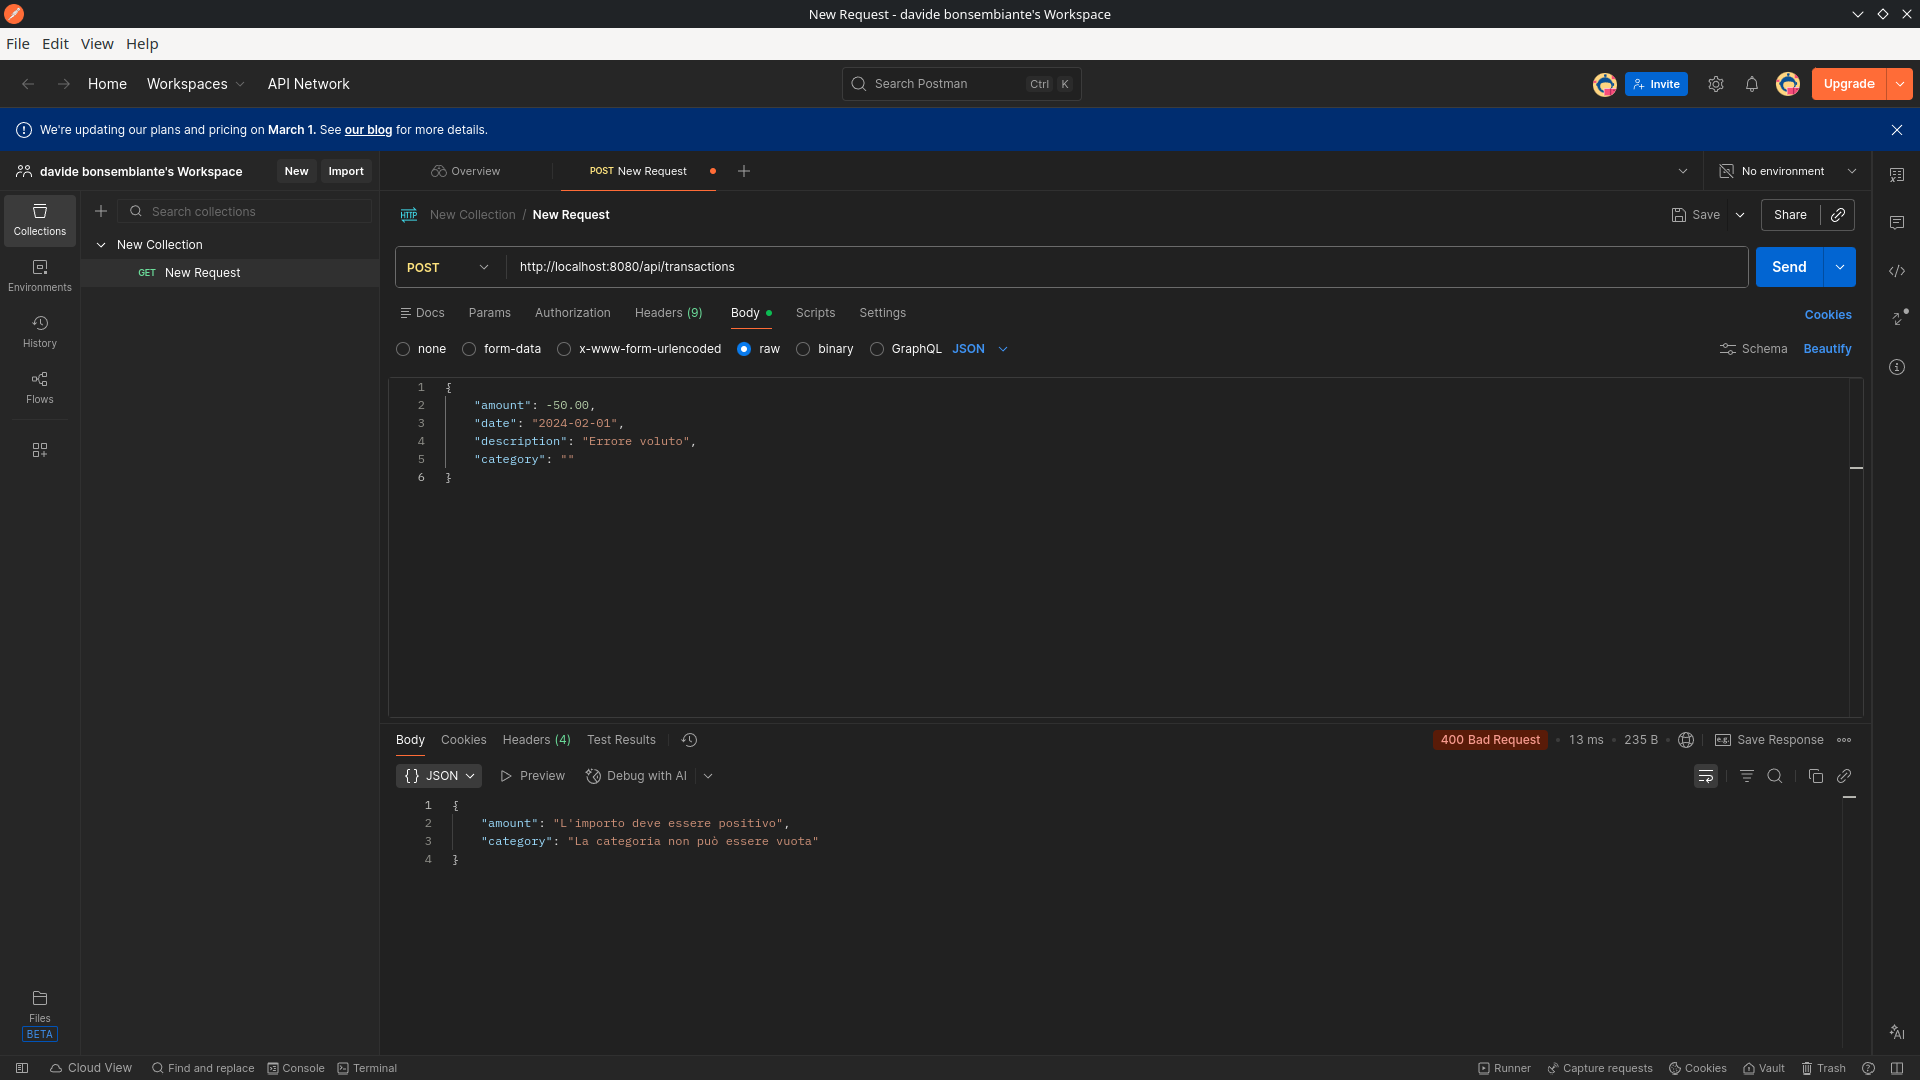
\includegraphics[width=1\textwidth]{../Iterazione_1/images/postman_bad_request.png}
    \caption{Test di validazione: risposta 400 Bad Request su importo negativo.}
    \label{fig:post_bad}
\end{figure}

\section{Conclusione Iterazione 1}

L'Iterazione 1 ha consegnato un microservizio di Accounting pienamente operativo e testato. L'adozione di Docker ha semplificato il deployment del database, mentre l'uso di pattern avanzati (DTO, Mapper, Global Exception Handling) ha garantito una codebase manutenibile e robusta. Il sistema è ora pronto per la successiva integrazione con i moduli di Analytics e Natural Language Understanding.

% 5. Iterazione 2 (Analytics, Algoritmi, DDD)
\input{2_Chapters/05_iterazione_2.tex}

% 6. Iterazione 3 (NLU, Integrazione, UI) + Conclusioni
\chapter{Iterazione 3: API Gateway, Web UI e NLU Engine}
\label{chap:iterazione3}

\section{Obiettivi e Integrazione di Sistema}

L'Iterazione 3 segna il passaggio da una collezione di microservizi backend disgiunti a una piattaforma applicativa integrata. L'obiettivo primario è stato chiudere il cerchio architetturale, fornendo all'utente un punto di accesso unico e un'interfaccia naturale per interagire con i dati finanziari.

Le attività si sono concentrate su tre pilastri fondamentali:
\begin{itemize}
    \item \textbf{Centralizzazione dell'accesso}: Introduzione di un API Gateway per astrarre la topologia dei microservizi e risolvere le problematiche di CORS.
    \item \textbf{Interfaccia Utente (Web UI)}: Sviluppo di un frontend server-side (Thymeleaf) integrato con le API di riconoscimento vocale del browser.
    \item \textbf{Intelligenza Semantica (NLU)}: Implementazione di un motore deterministico per la traduzione del linguaggio naturale in comandi transazionali strutturati.
\end{itemize}

\section{API Gateway: Centralizzazione del Routing}

Nelle iterazioni precedenti, i servizi rispondevano su porte diverse (\texttt{8081}, \texttt{8082}), costringendo il client a conoscere la topologia della rete. Per disaccoppiare il frontend dal backend, è stato introdotto il microservizio \texttt{jarfin-api-gateway}, basato su Spring Cloud Gateway.

\subsection{Configurazione Dichiarativa delle Rotte}
Il Gateway espone un unico entry-point sulla porta 8080 e instrada le richieste ai servizi interni tramite regole definite nel file \texttt{application.yml}.

\begin{lstlisting}[language=yaml, label={lst:gateway_yml}]
server:
  port: 8080
spring:
  cloud:
    gateway:
      routes:
        # Rotta verso il Core Accounting
        - id: accounting-service
          uri: http://localhost:8081
          predicates:
            - Path=/api/transactions/**

        # Rotta verso la Business Intelligence
        - id: analytics-service
          uri: http://localhost:8082
          predicates:
            - Path=/api/analytics/**

        # Rotta verso il Frontend (Web UI)
        - id: web-ui
          uri: http://localhost:8083
          predicates:
            - Path=/**
\end{lstlisting}

Questa configurazione implementa il pattern \textbf{Reverse Proxy}: il browser dialoga esclusivamente con \texttt{localhost:8080}, ignorando l'esistenza dei servizi sottostanti. Questo semplifica la gestione della sicurezza e centralizza il logging delle richieste.

\section{Web UI e Riconoscimento Vocale Ibrido}

L'interfaccia utente è stata sviluppata utilizzando \textbf{Thymeleaf} e \textbf{Bootstrap 5}, servita dal microservizio \texttt{jarfin-web-ui}.
Una scelta architetturale critica ha riguardato l'implementazione del riconoscimento vocale (Speech-to-Text).

\subsection{Strategia "Edge AI" (Client-Side Processing)}
Invece di inviare flussi audio pesanti al server (che richiederebbero larghezza di banda e costose GPU per la trascrizione), si è optato per l'utilizzo delle \textbf{Web Speech API} native del browser.
La trascrizione avviene localmente sul dispositivo dell'utente (Edge), e solo il testo risultante viene inviato al backend.

Nel file \texttt{index.html}, la logica JavaScript gestisce il ciclo di vita del microfono e l'attivazione tramite "Wake Word" ("Johnny"):

\begin{lstlisting}[language=JavaScript, label={lst:js_stt}]
recognition.onresult = (event) => {
    // Concatenazione risultati parziali
    let transcript = "";
    for (let i = event.resultIndex; i < event.results.length; ++i) {
        if (event.results[i].isFinal) 
            transcript += event.results[i][0].transcript.toLowerCase();
    }
    
    // Rilevamento Wake Word locale
    if (!isJarfinActivated && WAKE_WORDS.some(w => transcript.includes(w))) {
        activateJohnny(); // Attiva la UI di ascolto
    } 
    // Invio comando al backend
    else if (isJarfinActivated) {
        sendToBackend(transcript.trim());
    }
};
\end{lstlisting}

Questa architettura ibrida garantisce \textbf{latenza zero} nell'attivazione e maggiore \textbf{privacy}, poiché l'audio raw non lascia mai il dispositivo dell'utente.

\newpage

% SONO ARRIVATO QUA

\section{Natural Language Understanding (NLU) Engine}

Il cuore intelligente del sistema è il servizio \texttt{NaturalLanguageService}. A differenza degli approcci basati su LLM (Large Language Models), che sono probabilisticamente corretti ma lenti e costosi, JarFin adotta un motore **deterministico basato su regole**.

Questa scelta garantisce:
\begin{itemize}
    \item \textbf{Velocità}: Elaborazione in $O(N)$.
    \item \textbf{Affidabilità}: A parità di input, l'output è sempre identico.
    \item \textbf{Interpretabilità}: Ogni estrazione è giustificata da una regola regex o keyword.
\end{itemize}

\subsection{Implementazione: Regex e Keyword Mapping}
Il servizio utilizza espressioni regolari pre-compilate per l'estrazione di importi e ID, e una mappa hash per la classificazione semantica.

\begin{lstlisting}[language=Java, caption={Costanti e Pattern nel NaturalLanguageService}, label={lst:nlu_constants}]
private static final Pattern NUMBER_PATTERN = 
    Pattern.compile("(\\d+([.,]\\d{1,2})?)"); // Supporta 10.50 e 10,50
    
private static final Pattern DELETE_CMD = 
    Pattern.compile("(elimina|cancella|rimuovi|togli)", Pattern.CASE_INSENSITIVE);

private static final Map<String, String> CATEGORY_MAP = new HashMap<>();
static {
    CATEGORY_MAP.put("mcdonald", "Ristorante");
    CATEGORY_MAP.put("benzina", "Trasporti");
    // ... mappatura estesa di oltre 50 keyword
}
\end{lstlisting}

\section{Design in Piccolo: Analisi dell'Algoritmo NLU}

L'algoritmo di parsing (\texttt{parse}) trasforma una stringa naturale non strutturata in un oggetto \texttt{ParsedTransaction} pronto per il database.

\subsection{Pseudocodice Formale}
L'algoritmo segue una pipeline sequenziale di estrazione e pulizia.

\begin{lstlisting}[mathescape=true, caption={Pseudocodice Parser NLU}, label={lst:pseudocode_nlu}, basicstyle=\small\ttfamily]
Algoritmo ParseNaturalLanguage(text):
    Input: Stringa $S$ (comando utente)
    Output: Oggetto $T$ (Transazione strutturata) o NULL

    // 1. Pre-validazione
    IF $S$ is NULL OR length($S$) < 2 OR contains(STOP_WORDS, $S$) THEN
        RETURN NULL
    END IF
    $S_{lower} \leftarrow$ ToLowerCase($S$)

    // 2. Identificazione Intento (Command Classification)
    IF Match($P_{delete}$, $S$) THEN 
        $T.command \leftarrow$ DELETE
        $T.targetId \leftarrow$ ExtractId($S$)
    ELSE IF Match($P_{update}$, $S$) THEN
        $T.command \leftarrow$ UPDATE
        $T.targetId \leftarrow$ ExtractId($S$)
    ELSE
        $T.command \leftarrow$ CREATE
        $T.date \leftarrow$ CurrentDate()
    END IF

    // 3. Estrazione Importo (Regex)
    Match $M_{num} \leftarrow$ Find($P_{number}$, $S$ without IDs)
    IF $M_{num}$ found THEN
        $T.amount \leftarrow$ ParseDecimal($M_{num}.value$)
    END IF

    // 4. Classificazione Categoria (Keyword Matching)
    FOR each ($Key$, $Cat$) in $Map_{categories}$ DO:
        IF $S_{lower}$ contains $Key$ THEN
            $T.category \leftarrow Cat$
            BREAK // Match trovato (Priority First)
        END IF
    END FOR

    // 5. Pulizia Descrizione (Stop-word Removal)
    $T.description \leftarrow$ CleanText($S_{lower}$) 
    IF $T.description$ is empty THEN
        $T.description \leftarrow T.category$ OR "Generale"
    END IF

    RETURN $T$
\end{lstlisting}

\subsection{Analisi della Complessità Computazionale}
Analizziamo il costo temporale $T(n)$ dell'algoritmo, dove $n$ è la lunghezza della stringa di input.

\begin{enumerate}
    \item \textbf{Regex Matching}: L'applicazione di pattern regex semplici (senza backtracking annidato o ricorsivo) su una stringa di lunghezza $n$ ha complessità lineare $O(n)$.
    \item \textbf{Keyword Matching}: L'algoritmo itera su una mappa di $K$ parole chiave. Per ogni parola chiave, l'operazione `contains` ha un costo proporzionale alla lunghezza della stringa.
    \[ T_{match} \approx K \cdot O(n) \]
    Poiché $K$ è una costante di configurazione (circa 50 entry) e non dipende dall'input utente, asintoticamente questo termine si riduce a $O(n)$.
    \item \textbf{Clean Text}: La rimozione delle stop-word avviene tramite una serie di \texttt{replaceAll}, ciascuno dei quali scorre la stringa una volta.
    \[ T_{clean} = \sum_{regex} O(n) \approx C \cdot O(n) \]
\end{enumerate}

\textbf{Complessità Totale}:
\[ T(n) = O(n) + K \cdot O(n) + C \cdot O(n) \]
\[ T(n) = O(n) \]

L'algoritmo è **Lineare**. Questo garantisce che il tempo di elaborazione sia trascurabile (< 1ms) per frasi di lunghezza standard (es. 10-100 caratteri), rendendo l'esperienza utente percepita come "istantanea".

\section{Orchestrazione: CommandController}

Il \texttt{CommandController} funge da orchestratore backend. Riceve il testo dal frontend, invoca il servizio NLU e instrada il comando strutturato verso l'API Gateway.

Il metodo \texttt{processVoiceCommand} gestisce la logica di fallback e l'invio al Core Accounting:

\begin{lstlisting}[language=Java, caption={Processamento comando vocale}, label={lst:command_controller}]
@PostMapping("/process")
public ResponseEntity<?> processVoiceCommand(@RequestBody Map<String, String> payload) {
    String text = payload.get("text");
    ParsedTransaction parsed = nluService.parse(text);

    // Instradamento dinamico basato sul tipo di comando
    switch (parsed.getCommandType()) {
        case CREATE:
            // Fallback: se la categoria non e' dedotta, usa "Altro"
            if (parsed.getCategory() == null) parsed.setCategory("Altro");
            if (parsed.getAmount() == null) parsed.setAmount(BigDecimal.ZERO);
            
            // Chiamata all'Accounting Service via Gateway
            restTemplate.postForEntity(gatewayUrl + "/api/transactions", 
                                       parsed, Object.class);
            break;
            
        case DELETE:
            // Logica di eliminazione transazione
            break;
    }
    return ResponseEntity.ok(Map.of("message", "Salvato"));
}
\end{lstlisting}

\section{Strategia di Validazione e Testing}

Allo stato attuale dello sviluppo, la validazione dell'Iterazione 3 è in fase di completamento. Di seguito viene illustrata la **Strategia di Test** progettata per garantire la robustezza dei nuovi componenti integrati.

\subsection{Unit Testing: NLU Engine}
L'obiettivo primario è verificare la precisione dell'algoritmo di parsing. Sono previsti test parametrizzati con JUnit 5 per coprire i seguenti scenari:
\begin{itemize}
    \item \textbf{Scenario Base}: Input "Ho speso 10 euro per pizza" $\rightarrow$ \texttt{Amount=10.00}, \texttt{Category=Ristorante}.
    \item \textbf{Edge Case}: Input con separatori decimali diversi ("10.50", "10,50") o valute miste.
    \item \textbf{Comandi Complessi}: "Elimina la transazione 42" $\rightarrow$ \texttt{Command=DELETE}, \texttt{TargetId=42}.
    \item \textbf{Input "Sporchi"}: Frasi lunghe con molte stop-word per verificare l'efficacia del metodo \texttt{cleanText}.
\end{itemize}

\subsection{Integration Testing: Gateway e Controller}
Per validare l'orchestrazione, verranno eseguiti test di integrazione che coinvolgono il container del Gateway:
\begin{itemize}
    \item \textbf{Routing Test}: Verifica che le chiamate a \texttt{localhost:8080/api/transactions} vengano correttamente inoltrate al servizio Accounting.
    \item \textbf{Flow Test}: Simulazione di una chiamata POST al \texttt{CommandController} con un payload testuale, verificando che l'Accounting Service riceva correttamente l'oggetto JSON strutturato.
\end{itemize}

Questa fase di Quality Assurance, attualmente in corso, certificherà la stabilità della piattaforma prima del rilascio finale.

\section{Conclusione Iterazione 3}

L'Iterazione 3 ha completato l'architettura JarFin.
L'API Gateway ha fornito un layer di astrazione essenziale per la sicurezza e il routing.
Il motore NLU, grazie alla sua natura algoritmica $O(n)$, offre un'alternativa robusta e performante all'IA generativa per compiti strutturati, garantendo un'esperienza utente fluida e priva di latenze significative.


% 8. Conclusioni
\input{2_Chapters/07_conclusioni.tex}

% ==============================
% BIBLIOGRAFIA
% ==============================
\newpage
\nocite{*}

\bibliographystyle{IEEEtran}
\bibliography{bibliography}

\end{document}